%----------------------------------------------------------------------------------------
% Preambulo y Configuración
%----------------------------------------------------------------------------------------

\documentclass[
    11pt,
    spanish,
    singlespacing,
    parskip,
    headsepline,
    bookmarks=true,
    unicode=true,
    pdftoolbar=true,
    pdfmenubar=true,
    pdffitwindow=false,
    colorlinks=true,
    linkcolor=blue,
    citecolor=blue,
    urlcolor=blue
]{MastersDoctoralThesis}

\usepackage[utf8]{inputenc} % Codificación de entrada UTF-8
\usepackage[T1]{fontenc}    % Codificación de salida para caracteres especiales
\usepackage{graphicx}       % Manejo de gráficos
\usepackage{eso-pic}        % Permite agregar fondos
\usepackage{hyperref}       % Manejo de hipervínculos y marcadores
\usepackage{amsmath}        % Formulas matematicas
\usepackage{float}

% Redefinición de caracteres problemáticos en marcadores
\hypersetup{
    pdftitle={Título del Documento},
    pdfauthor={Autor del Documento},
    pdfkeywords={Sistemas Embebidos, Internet de las Cosas, Inteligencia Artificial},
    pdfstartview={FitH},
    unicode=true,
    colorlinks=true,
    linkcolor=blue,
    citecolor=blue,
    urlcolor=blue
}

\pdfstringdefDisableCommands{%
  \def\texttt#1{#1}%
  \def\textbf#1{#1}%
  \def\textit#1{#1}%
  \def\"{\"}%
  \def\~{~}%
  \def\'{'}%
  \def\^{}%
  \def\textunderscore{\_} % Manejo del subrayado en marcadores
}


% Definir comandos requeridos por la clase
\newcommand{\degreename}{Maestría en Ciencias} % Cambia según tu título
\newcommand{\univname}{Universidad Nacional de Ejemplo} % Cambia según tu universidad
\newcommand{\keywordnames}{Palabras clave:}
%----------------------------------------------------------------------------------------
% Documento Principal
%----------------------------------------------------------------------------------------

\begin{document}

% Configuración de la portada
\posgrado{Carrera / Maestría}
\keywords{Sistemas Embebidos, Internet de las Cosas, Inteligencia Artificial}

% Incluir la portada desde un archivo separado
%----------------------------------------------------------------------------------------
% PORTADA
%----------------------------------------------------------------------------------------
\begin{titlepage}
    % Fondo completo con el PDF que incluye la barra y el logo
    \AddToShipoutPictureBG*{
\includegraphics[width=\paperwidth, height=\paperheight]{Figures/fondo.pdf}}

    % Contenido principal
    \begin{flushright}
        \setlength{\rightskip}{-2cm} % Ajusta la sangría derecha
        \vspace*{7.5cm} % Ajustar según la posición vertical deseada

        % Título
        {\fontfamily{phv}\bfseries\fontsize{33pt}{40pt}\selectfont
        Integración de Técnicas de Visión Computacional y Aprendizaje Automático en un Robot Militar para la Identificación y Eliminación Eficiente de Objetivos} \\[1.5cm]

        % Autor
        {\fontfamily{phv}\fontsize{20pt}{25pt}\selectfont
        \small{Lucas Martín Gaggino}
        \\
        \small{Tomas Jesús Contessi}} \\[1cm]

        % Carrera o Maestría (comentar o descomentar la línea correspondiente)
        {\fontfamily{phv}\fontsize{15pt}{20pt}\selectfont
        \textbf{Trabajo Profesional}
        \\
        \textbf{Carrera de Ingeniería Electrónica}
        % \textbf{Carrera de Especialización en Internet de las Cosas} \\
        % \textbf{Carrera de Especialización en Inteligencia Artificial} \\
        % \textbf{Maestría en Sistemas Embebidos} \\
        % \textbf{Maestría en Internet de las Cosas} \\
        % \textbf{Maestría en Inteligencia Artificial Embebida} \\
        % \textbf{Maestría en Computación de Borde} \\
        % \textbf{Maestría en Inteligencia Artificial} \\
        } \\[2cm]

        % Director
        {\fontfamily{phv}\fontsize{11pt}{15pt}\selectfont
        \textbf{Tutor:} Federico G. Zacchigna} \\[1cm]

        % Jurados
        %{\fontfamily{phv}\fontsize{11pt}{15pt}\selectfont
        %\textbf{Jurados:}} \\[0.5cm]
        %{\fontfamily{phv}\fontsize{11pt}{15pt}\selectfont
        %Jurado 1 (pertenencia)} \\ 
        %{\fontfamily{phv}\fontsize{11pt}{15pt}\selectfont
        %Jurado 2 (pertenencia)} \\ 
        %{\fontfamily{phv}\fontsize{11pt}{15pt}\selectfont
        %Jurado 3 (pertenencia)} \\[2cm]

        % Fecha y lugar
        {\fontfamily{phv}\itshape\fontsize{10pt}{12pt}\selectfont
        Ciudad de Buenos Aires, Agosto de 2025} % Ejemplo: Ciudad de Córdoba, junio de 2025
    \end{flushright}
\end{titlepage}


% Configuración del contenido preliminar
\frontmatter % Usar numeración romana para las páginas preliminares
\pagestyle{plain} % Estilo de encabezado simple

%----------------------------------------------------------------------------------------
% Resumen
%----------------------------------------------------------------------------------------

\begin{abstract}
\addchaptertocentry{\abstractname} % Agregar resumen al índice
Este trabajo profesional presenta el desarrollo de un sistema robótico militar autónomo capaz de identificar y neutralizar objetivos aéreos de manera eficiente mediante el uso de inteligencia artificial y visión por computadora. El sistema integra capacidades de navegación autónoma, reconocimiento de objetivos en tiempo real y control automático de armamento, coordinados por una arquitectura de software modular que permite la operación independiente y escalable de cada componente. La principal innovación del proyecto radica en la combinación de técnicas de aprendizaje automático con un entorno de simulación avanzado que permite entrenar y validar los algoritmos de manera segura y económica, superando las limitaciones tradicionales de desarrollo en entornos militares reales.

Los resultados demuestran que el sistema desarrollado puede operar de manera autónoma en diversos escenarios, navegando eficientemente mientras detecta y neutraliza objetivos con alta precisión. La importancia de este trabajo reside en su contribución al desarrollo de sistemas de defensa inteligentes que pueden reducir significativamente los riesgos para el personal militar y mejorar la efectividad operacional. El lector encontrará en esta memoria una descripción completa del proceso de desarrollo, desde la conceptualización teórica hasta la implementación práctica y validación experimental, incluyendo tanto el diseño del hardware como el desarrollo del software de control. El proyecto integra conocimientos fundamentales de la ingeniería electrónica, incluyendo sistemas de control, procesamiento de señales, programación de sistemas embebidos y diseño de circuitos, demostrando la aplicación práctica de estos conceptos en una solución tecnológica innovadora para aplicaciones de defensa.




\end{abstract}

%----------------------------------------------------------------------------------------
% Agradecimientos
%----------------------------------------------------------------------------------------

%\begin{acknowledgements}
%\vspace{1.5cm}
%Esta sección es para agradecimientos personales y es totalmente \textbf{OPCIONAL}.
%\end{acknowledgements}

%----------------------------------------------------------------------------------------
% Índice
%----------------------------------------------------------------------------------------

\tableofcontents
\listoffigures
\listoftables

%----------------------------------------------------------------------------------------
% Dedicatoria
%----------------------------------------------------------------------------------------

%\dedicatory{\textbf{Dedicado a... [OPCIONAL]}}

%----------------------------------------------------------------------------------------
% Capítulos
%----------------------------------------------------------------------------------------

\mainmatter % Iniciar numeración numérica para el contenido principal
\pagestyle{thesis} % Estilo de encabezado de tesis

% Incluir capítulos desde archivos separados
\chapter{Presentación}

\label{Chapter:Presentacion} 

\section{Introducción}
\label{Introduccion}

En los últimos años, los drones han emergido como herramientas clave en los conflictos bélicos modernos, representando una evolución significativa en la tecnología militar. Particularmente en el contexto de la guerra Ruso-Ucraniana, estos dispositivos han sido adoptados ampliamente como armas de guerra, destacándose por su precisión, versatilidad y relativo bajo costo en comparación con los sistemas tradicionales. Sin embargo, esta innovación tecnológica también ha expuesto vulnerabilidades en los sistemas de defensa actuales, los cuales no han logrado ser completamente efectivos frente a esta nueva amenaza.

La principal debilidad de las defensas convencionales radica en su incapacidad para contrarrestar la precisión y la adaptabilidad de los drones, así como en el elevado costo asociado al despliegue y mantenimiento de sistemas de misiles antiaéreos. En este contexto, surge la necesidad imperiosa de desarrollar soluciones innovadoras que permitan identificar y neutralizar estas amenazas de manera eficiente y económica. 

El presente trabajo aborda esta problemática mediante la integración de técnicas avanzadas de visión computacional y aprendizaje automático en un robot militar, diseñado para operar en entornos hostiles. Este enfoque busca optimizar la detección y eliminación de objetivos, ofreciendo una alternativa robusta y efectiva a los sistemas de defensa tradicionales.


\section{Antecedentes}
\label{Antecedentes}

Los drones comerciales comenzaron a utilizarse a gran escala en el conflicto Ruso-Ucraniano en el año 2022, marcando un punto de inflexión en el uso de tecnología accesible y versátil en el campo de batalla. Este fenómeno no solo subraya la capacidad de los drones para adaptarse rápidamente a las necesidades militares, sino que también refleja una tendencia histórica en la evolución de los sistemas de armas y defensa.

La historia de la guerra es, en esencia, una constante evolución entre las herramientas ofensivas y los mecanismos defensivos. Durante la Edad Media, los castillos representaban una defensa formidable contra los ejércitos a pie, proporcionando refugio y ventajas estratégicas. Sin embargo, la invención de la pólvora y el desarrollo de cañones y armas de fuego hicieron obsoletos tanto a los castillos como a las armaduras tradicionales, redefiniendo las estrategias de combate.

De manera similar, los avances en los misiles antiaéreos impulsaron la evolución de los aviones de combate, dando lugar a modelos como el SR-71 Blackbird, diseñado para superar los sistemas de defensa convencionales mediante su velocidad y altitud extremas. Ahora, los drones han emergido como una alternativa altamente económica y fácil de desplegar, con la capacidad de infligir daño localizado tanto a personal como a vehículos. Esta nueva generación de tecnología bélica permite a los combatientes alcanzar objetivos estratégicos con precisión y a un costo significativamente menor en comparación con los sistemas tradicionales.

El conflicto en Ucrania ha puesto de manifiesto estas tendencias, demostrando cómo los drones pueden ser utilizados tanto para vigilancia como para ataques precisos, consolidando su posición como una herramienta clave en los conflictos modernos.
\section{Estado del Arte}
\label{Estado del Arte}

En la actualidad, los drones han transformado profundamente la dinámica de los conflictos bélicos, como se ha evidenciado en la guerra Ruso-Ucraniana. En los primeros días del conflicto, una de las estrategias defensivas más comunes contra los drones operados remotamente por pilotos consistía en que los soldados dispararan directamente hacia ellos. Sin embargo, esta táctica demostró ser poco efectiva, con tasas de acierto extremadamente bajas debido a la velocidad y maniobrabilidad de los drones.

Para mitigar los daños ocasionados por estos dispositivos, los vehículos comenzaron a incluir mayores niveles de armadura. Este enfoque condujo al renacimiento del concepto del "tanque tortuga", el cual consiste en la adición de armadura separada del casco principal del tanque. Este diseño busca disipar las explosiones generadas por los drones, protegiendo las partes más expuestas del vehículo.

Históricamente, los tanques como el T-72, de diseño ruso, y los modelos modernos americanos, como el M1 Abrams y el M2 Bradley, fueron concebidos principalmente para enfrentamientos directos contra otros tanques, en un contexto de posible guerra entre Rusia y Estados Unidos. Alternativamente, también se diseñaron para conflictos de "contrainsurgencia", combates contra fuerzas irregulares de países con recursos limitados. No obstante, la guerra a gran escala (LSCO, por sus siglas en inglés, "Large Scale Conflict") que se está desarrollando en Ucrania ha demostrado que estos diseños enfrentan desafíos significativos frente a las tácticas modernas que emplean drones.

Una característica clave de los drones empleados en el conflicto es que operan a través del espectro radioeléctrico, utilizando frecuencias de 390-510 MHz y 750-1050 MHz. Como contramedida, se han desplegado "jammers" o bloqueadores de señal para inutilizar las comunicaciones entre los drones y sus operadores. Sin embargo, esta medida ha llevado a una carrera armamentista tecnológica, donde nuevos protocolos de comunicación se desarrollan continuamente para permitir que los drones puedan evadir estas interferencias.

En este contexto, una innovación destacable ha sido la implementación de drones rusos controlados mediante fibra óptica. Esta tecnología los hace completamente inmunes a los bloqueadores de señal, ya que elimina la dependencia del espectro radioeléctrico. Este avance representa un salto tecnológico significativo en el uso de drones en el campo de batalla, consolidando su papel como un componente esencial en las estrategias modernas de guerra.
\section{Áreas Profesionales de Relevancia}
\label{Áreas Profesionales de Relevancia}

\begin{itemize}
    \item Ingeniería Electrónica
    \item Visión Computacional
    \item Inteligencia Artificial y Aprendizaje Automático
    \item Ingeniería Mecánica
    \item Ingeniería de Telecomunicaciones
    \item Diseño de Sistemas Embebidos
    \item Fabricación y Prototipado
\end{itemize}

\chapter{Alcance y Objetivos}

\label{Chapter:Alcance y Objetivos}


En este capítulo se definen los alcances y objetivos del proyecto, estableciendo el marco de trabajo y las metas específicas que guían el desarrollo del sistema robótico militar autónomo. Los objetivos se estructuran en un objetivo general y objetivos específicos, mientras que los alcances delimitan el ámbito de aplicación y las limitaciones del trabajo.



\section{Objetivos generales}
\label{Objetivos generales}

\begin{itemize}
    
    
    \item \textbf{Desarrollar un sistema de entrenamiento virtual:} Este objetivo implica la creación de un sistema completo de entrenamiento virtual que integre herramientas de simulación avanzadas y algoritmos de aprendizaje automático. Se busca no solo diseñar escenarios virtuales realistas, sino también implementar un entorno interactivo que permita al robot militar aprender y adaptarse a diferentes situaciones de combate simuladas.
    
    
    \item \textbf{Construir un prototipo físico del robot militar:} Desarrollar un prototipo físico del robot basado en los resultados obtenidos de los entrenamientos virtuales. Este prototipo servirá como herramienta para validar y complementar los resultados virtuales con pruebas prácticas en condiciones controladas, permitiendo ajustes y mejoras en el diseño y rendimiento del robot.
    
    
    \item \textbf{Integrar simulación virtual con validación física para garantizar robustez:} Combina la simulación virtual con la validación física para asegurar la robustez y efectividad del sistema en situaciones reales de combate. Este enfoque integral garantiza que el robot esté completamente preparado para enfrentar los desafíos del campo de batalla, al haber sido entrenado y validado tanto en entornos virtuales como físicos.

    \item \textbf{ Describir un proceso de producción para un prototipo productivo:} Este objetivo implica detallar las etapas necesarias para la producción de un prototipo funcional. Incluye definir el diseño preliminar, seleccionar componentes, integrar subsistemas de hardware y software, desarrollar e implementar algoritmos para navegación y control, ensamblar el prototipo con componentes electrónicos y mecánicos.


    
\end{itemize}
\section{Objetivos particulares}
\label{Objetivos particulares}

\begin{itemize}
    \item \textbf{Implementar algoritmos de navegación:} Crear algoritmos avanzados que permitan al robot moverse de manera autónoma y eficiente en diferentes entornos, asegurando su capacidad para evitar obstáculos y alcanzar objetivos específicos.
    
    \item \textbf{Utilizar técnicas de IA para detectar objetivos:} Aplicar algoritmos de inteligencia artificial que permitan al robot identificar y localizar objetivos de manera precisa, optimizando su capacidad de respuesta en tiempo real.

    \item \textbf{Integrar sensores y actuadores en el prototipo:}
    Incorporar y coordinar diversos sensores y actuadores en el prototipo del robot, permitiéndole interactuar de manera precisa con su entorno y recolectar datos esenciales para su funcionamiento y control.
    
    \item \textbf{Realizar pruebas y validación en entornos simulados:}
    Desarrollar y ejecutar un programa de pruebas exhaustivas en entornos virtuales simulados, asegurando que el robot esté preparado para enfrentar situaciones reales mediante ajustes y mejoras continuas basadas en los resultados obtenidos.
    
    \item \textbf{Realizar pruebas y validación en el prototipo físico:} Llevar a cabo una serie de pruebas exhaustivas en el prototipo físico del robot para evaluar su rendimiento en condiciones controladas. Estas pruebas incluirán la validación de su capacidad para detectar y eliminar objetivos de aproximadamente 45x45 centímetros a una distancia de 20 metros, así como la verificación de la integración y funcionamiento de los sensores, actuadores y sistemas de navegación.

    
\end{itemize}

\chapter{Introducción Teórica} % Main chapter title

\label{Chapter:Introducción Teórica} % Change X to a consecutive number; for referencing this chapter elsewhere, use \ref{ChapterX}
Este capítulo presenta los fundamentos teóricos que sustentan el desarrollo del sistema robótico militar autónomo. Se abordan los conceptos clave de cada tecnología implementada, desde la detección de imágenes mediante aprendizaje automático hasta los algoritmos de navegación y control, proporcionando el marco conceptual necesario para comprender las decisiones de diseño y la implementación del sistema.



\section{Detección de imágenes}
La detección de imágenes es un componente crucial en sistemas autónomos para la percepción del entorno y la identificación de objetos de interés. En el contexto de este proyecto, se centra en la detección específica de vehículos aéreos no tripulados (drones) hostiles. Para ello, se exploran algoritmos avanzados de visión computacional, capaces de procesar el flujo de video en tiempo real proveniente de las cámaras del robot.

Desde un punto de vista teórico, la detección de objetos se enmarca dentro del campo del aprendizaje profundo (\textit{deep learning}), particularmente mediante el uso de redes neuronales convolucionales (CNN, por sus siglas en inglés: Convolutional Neural Networks). Las CNN han demostrado un desempeño sobresaliente en tareas de visión computacional debido a su capacidad para aprender características jerárquicas directamente de los datos de imagen, eliminando la necesidad de ingeniería manual de características. Modelos como YOLO (You Only Look Once) y Faster R-CNN son ejemplos prominentes en la detección de objetos en tiempo real. YOLO, por ejemplo, reformula la detección como un problema de regresión, prediciendo simultáneamente las cajas delimitadoras (\textit{bounding boxes}) y las probabilidades de clase en una sola pasada de la red, lo que lo hace adecuado para aplicaciones donde la velocidad es crítica, como en este proyecto.

Adicionalmente, el sistema incorpora una funcionalidad de seguimiento por color (color tracking). Si bien la detección primaria de objetivos se basa en modelos más complejos, el seguimiento por color se presenta como una herramienta útil para tareas de \textit{troubleshooting}, calibración o incluso para el seguimiento de objetos cooperativos o marcadores específicos en el entorno. Este enfoque se basa en técnicas más tradicionales de procesamiento de imágenes, como la segmentación en el espacio de color HSV (Hue, Saturation, Value), que permite aislar regiones de interés basadas en tonalidades específicas, siendo robusto frente a variaciones de iluminación en comparación con el espacio RGB.

\begin{figure}[htbp]
\centering
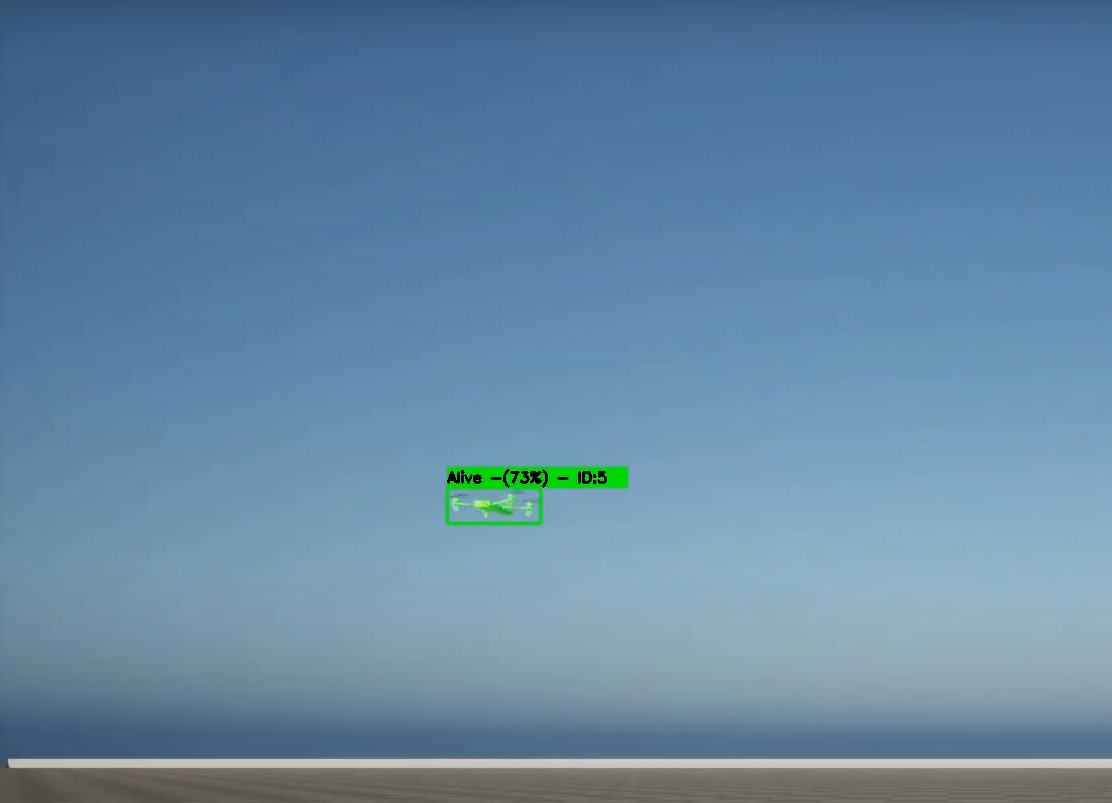
\includegraphics[width=.75\textwidth]{./Figures/deteccion_ejemplo.png}
\caption{Ejemplo de seguimiento por color.}
\label{fig:deteccion_ejemplo}
\end{figure}

El rendimiento y la robustez de los algoritmos de detección dependen en gran medida de la calidad y diversidad de los datos de entrenamiento. Por esta razón, se adopta una estrategia híbrida para la generación del conjunto de datos, combinando:
\begin{itemize}
    \item \textbf{Imágenes reales:} Capturadas en diversos escenarios y condiciones, representando fielmente el dominio de operación.
    \item \textbf{Imágenes sintéticas:} Generadas mediante el entorno de simulación desarrollado en Unreal Engine 5. Esta aproximación permite crear una gran variedad de situaciones, ángulos de visión, condiciones de iluminación y modelos de drones, superando las limitaciones logísticas y de costo asociadas a la recolección exclusiva de datos reales.
\end{itemize}

Un aspecto crítico en el entrenamiento de modelos de aprendizaje profundo es el fenómeno del \textit{overfitting}, donde el modelo aprende patrones específicos del conjunto de entrenamiento que no generalizan bien a datos nuevos. Para mitigar esto, se emplean técnicas de regularización como \textit{dropout}, aumento de datos (\textit{data augmentation}) y la mencionada incorporación de datos sintéticos, que enriquecen la variabilidad del conjunto de entrenamiento. Además, se considera el problema del desbalance de clases, ya que en escenarios reales los drones hostiles pueden ser menos frecuentes que otros objetos, lo que requiere estrategias como el muestreo ponderado o métricas de evaluación específicas como el F1-score.

\section{Mapeo}
El mapeo es el proceso mediante el cual un robot construye una representación espacial del entorno que lo rodea. Esta representación es fundamental para la navegación autónoma, permitiendo al robot localizarse a sí mismo y planificar rutas hacia un objetivo. En este proyecto, el robot está equipado con un sensor LIDAR (Light Detection and Ranging), que proporciona mediciones precisas de distancia a los objetos circundantes en forma de una nube de puntos.

\begin{figure}[htbp]
\centering
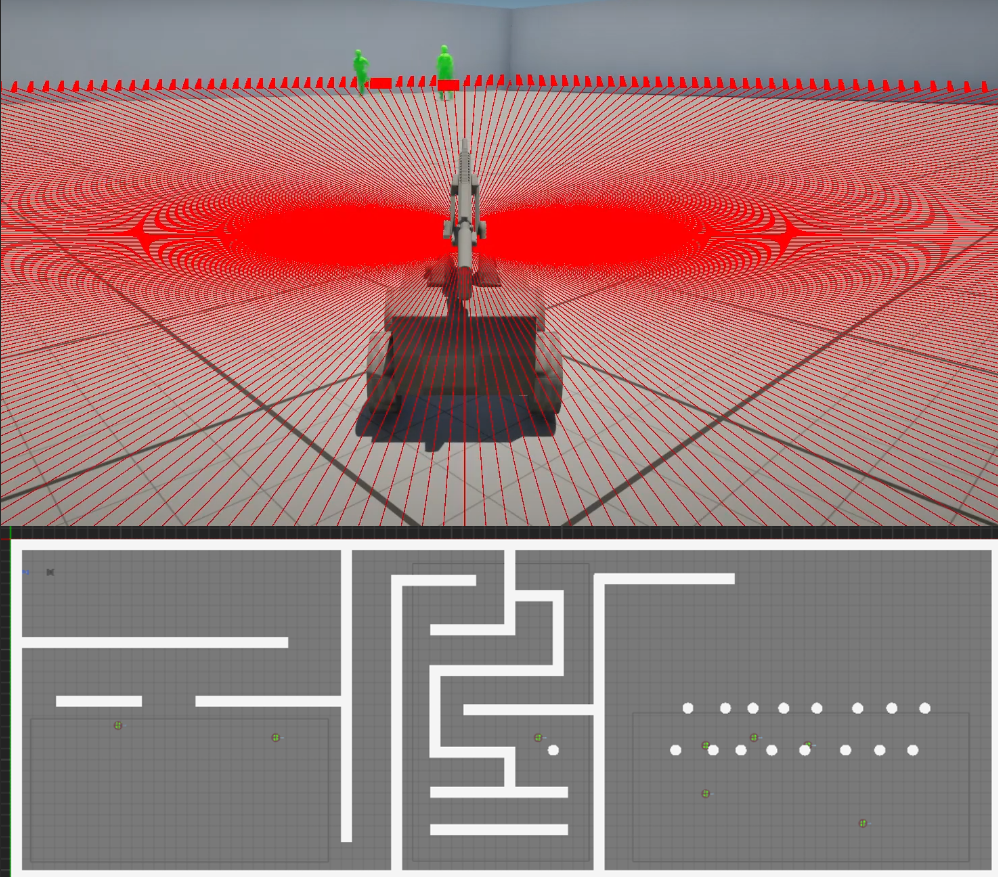
\includegraphics[width=.75\textwidth]{./Figures/mapeo_lidar_slam.png}
\caption{Ilustración del proceso de mapeo con LIDAR y SLAM.}
\label{fig:mapeo_lidar_slam}
\end{figure}

Para construir el mapa a partir de los datos del LIDAR y, simultáneamente, estimar la pose (posición y orientación) del robot dentro de ese mapa, se recurre a técnicas de SLAM (Simultaneous Localization and Mapping). El SLAM es un problema complejo, ya que la estimación de la pose del robot y la construcción del mapa son interdependientes. Desde un punto de vista teórico, el SLAM puede formularse como un problema de estimación bayesiana, donde se busca maximizar la probabilidad conjunta de la pose del robot y el mapa dado un conjunto de observaciones y controles. Esto implica modelar la incertidumbre inherente a las mediciones de los sensores y los errores acumulados en la odometría del robot.

Se investiga la aplicación de algoritmos eficientes de SLAM, con un enfoque particular en variantes como FastSLAM, que descompone el problema para mejorar la eficiencia computacional, especialmente en entornos de gran escala. FastSLAM utiliza un filtro de partículas para representar la incertidumbre en la pose del robot y mantiene estimaciones separadas para los \textit{landmarks} del entorno. Este enfoque combina las ventajas de los métodos basados en filtros de partículas con la eficiencia de los filtros de Kalman extendidos (EKF) para la estimación de \textit{landmarks}, reduciendo la complejidad computacional de $O(N^2)$ a $O(N \log M)$, donde $N$ es el número de partículas y $M$ el número de \textit{landmarks}. Además, se exploran enfoques más recientes como el SLAM basado en grafos (Graph-SLAM), que optimiza la trayectoria completa del robot y el mapa mediante la minimización de errores acumulados, siendo especialmente útil en entornos con bucles cerrados (\textit{loop closure}).

Un desafío adicional en el contexto militar es la operación en entornos dinámicos, donde objetos o personas pueden moverse, invalidando partes del mapa. Esto requiere la implementación de estrategias de actualización dinámica del mapa y la detección de cambios en el entorno, un área activa de investigación en el campo del SLAM.

\section{Path planning}
Una vez que el robot dispone de un mapa del entorno y conoce su ubicación, el siguiente paso es la planificación de rutas (path planning). Este proceso consiste en encontrar una trayectoria óptima o factible desde la posición actual del robot hasta un punto objetivo, evitando obstáculos y considerando otras restricciones (por ejemplo, el tipo de terreno o zonas prohibidas).

Para esta tarea, se implementa el algoritmo A* (A-star). A* es un algoritmo de búsqueda informada que encuentra el camino de menor costo entre un nodo inicial y un nodo objetivo en un grafo. Utiliza una función heurística para estimar el costo restante hasta el objetivo, lo que guía la búsqueda hacia las regiones más prometedoras del espacio de estados. Es ampliamente utilizado en robótica debido a su completitud (garantiza encontrar una solución si existe) y optimalidad (encuentra el camino de menor costo si la heurística es admisible). El mapa generado por el módulo SLAM sirve como base para la construcción del grafo sobre el cual opera A*.

Desde un punto de vista teórico, A* pertenece a la familia de algoritmos de búsqueda heurística y se deriva de la búsqueda de Dijkstra, pero incorpora una estimación del costo futuro (heurística) para priorizar los nodos a explorar. La función de evaluación de A* se define como $f(n) = g(n) + h(n)$, donde $g(n)$ es el costo acumulado desde el nodo inicial hasta el nodo $n$, y $h(n)$ es la heurística que estima el costo desde $n$ hasta el objetivo. Para garantizar la optimalidad, $h(n)$ debe ser admisible, es decir, nunca sobreestimar el costo real del camino restante. En este proyecto, se utiliza típicamente la distancia euclidiana o de Manhattan como heurística, dependiendo de la estructura del grafo que representa el mapa.

\begin{figure}[htbp]
\centering
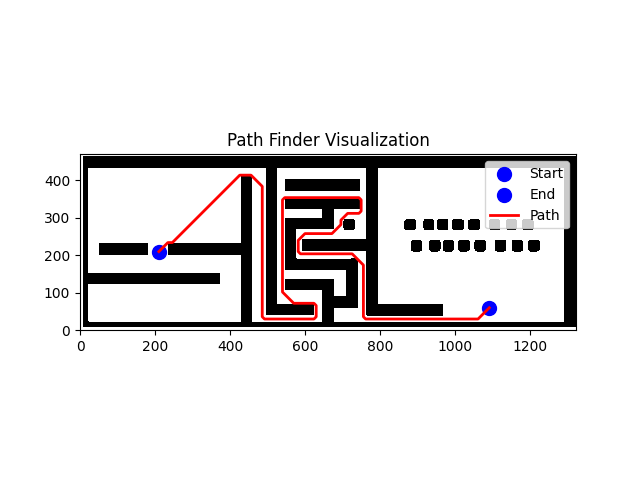
\includegraphics[width=.75\textwidth]{./Figures/path_planning_astar.png}
\caption{Ejemplo de planificación de ruta utilizando el algoritmo A*.}
\label{fig:path_planning_astar}
\end{figure}

Además de A*, existen otros enfoques para la planificación de rutas, como los algoritmos probabilísticos (por ejemplo, RRT - Rapidly-exploring Random Tree) que son más adecuados para espacios de alta dimensionalidad o entornos con obstáculos complejos. Sin embargo, A* se selecciona por su simplicidad de implementación y su eficacia en mapas discretizados, como los generados por SLAM. Un aspecto a considerar es la suavización de la trayectoria resultante, ya que A* puede generar caminos con cambios abruptos de dirección, no ideales para la dinámica de un robot físico. Para ello, se pueden aplicar técnicas de post-procesamiento como la interpolación de splines o algoritmos de suavizado basados en gradientes.

\section{Seguimiento de ruta}
Tras la planificación de una ruta, el robot debe ser capaz de seguirla con precisión. El seguimiento de ruta, también conocido como control de trayectoria o \textit{path tracking}, implica la implementación de algoritmos de control que ajustan continuamente los actuadores del robot (por ejemplo, velocidad y dirección de las ruedas o propulsores) para minimizar el error entre la posición actual del robot y la trayectoria deseada.

Existen diversas estrategias para el seguimiento de ruta, como los controladores PID (Proporcional-Integral-Derivativo), algoritmos de \textit{Pure Pursuit}, o técnicas basadas en modelos predictivos. La elección del controlador adecuado depende de la dinámica del robot, las características del entorno y los requisitos de precisión de la misión. El objetivo es asegurar que el robot se mantenga sobre la ruta planificada por A*, incluso ante perturbaciones o errores de estimación en su localización.

Teóricamente, el problema del seguimiento de ruta puede formularse como un problema de control óptimo, donde se busca minimizar una función de costo que representa el error de seguimiento y, potencialmente, otras variables como el consumo de energía o la suavidad del movimiento. Los controladores PID son una solución ampliamente utilizada debido a su simplicidad y robustez. Un controlador PID calcula la acción de control como una combinación lineal de tres términos: el error proporcional (P), la integral del error acumulado (I) para eliminar errores estacionarios, y la derivada del error (D) para anticipar cambios en el error. Sin embargo, los PID requieren un ajuste cuidadoso de sus parámetros (ganancias $K_p$, $K_i$, $K_d$) para cada sistema específico, lo que puede ser un proceso iterativo.

Por otro lado, el algoritmo \textit{Pure Pursuit} es un método geométrico que calcula un punto de mira (\textit{lookahead point}) en la trayectoria deseada, a una distancia fija del robot, y ajusta la dirección para alcanzarlo. Este enfoque es intuitivo y fácil de implementar, pero su desempeño depende críticamente de la elección de la distancia de anticipación, que debe balancear la estabilidad (distancias largas) con la precisión en curvas cerradas (distancias cortas). Finalmente, los controladores basados en modelos predictivos (MPC, Model Predictive Control) representan un enfoque más avanzado, donde se utiliza un modelo dinámico del robot para predecir su comportamiento futuro y optimizar las acciones de control en un horizonte de tiempo finito. Aunque computacionalmente más costoso, el MPC es capaz de manejar restricciones explícitas y dinámicas no lineales, siendo ideal para robots con comportamientos complejos.

\section{Simulación}
La simulación desempeña un papel fundamental en el desarrollo y validación de sistemas robóticos complejos, especialmente aquellos destinados a operar en entornos dinámicos o peligrosos. Permite probar algoritmos, evaluar diseños y realizar experimentos de forma segura, rápida y económica antes de realizar pruebas en el hardware físico.

Como se detalló en la Sección \ref{sec:simulador} , este proyecto utiliza Unreal Engine 5 (UE5) como plataforma de simulación. La elección de UE5 se justifica por su capacidad para generar entornos 3D realistas, simular físicas complejas y emular sensores como cámaras y LIDAR con alta fidelidad. Esto es esencial para:
\begin{itemize}
    \item Validar los algoritmos de percepción (detección de imágenes, SLAM).
    \item Probar y refinar los algoritmos de planificación y seguimiento de ruta en diversos escenarios.
    \item Generar datos sintéticos para el entrenamiento de modelos de aprendizaje automático, como se mencionó anteriormente.
    \item Realizar pruebas de integración del sistema completo en un entorno controlado.
\end{itemize}
El uso de un simulador avanzado como UE5 acelera significativamente el ciclo de desarrollo, permite la exploración de un mayor número de escenarios y contribuye a la robustez general del sistema robótico.

Desde una perspectiva teórica, la simulación en robótica se basa en la creación de modelos matemáticos y computacionales que aproximan el comportamiento del mundo real. Esto incluye la modelización de la dinámica del robot (cinemática y dinámica), las interacciones con el entorno (colisiones, fricción) y el ruido de los sensores. Un desafío clave es el \textit{reality gap}, la discrepancia entre el comportamiento simulado y el real, que puede limitar la transferibilidad de los resultados de la simulación al hardware físico. Para minimizar este problema, UE5 permite la incorporación de ruido sintético en las mediciones de los sensores y la simulación de condiciones ambientales variables, acercando el entorno virtual al real. Además, técnicas como el aprendizaje por transferencia (\textit{transfer learning}) y la adaptación al dominio (\textit{domain adaptation}) se utilizan para ajustar los modelos entrenados en simulación a datos del mundo real.


\chapter{Analisis técnico}

\label{Analisis técnico}

\section{sección 1}
\section{sección 2}



\chapter{Analisis de mercado}

\label{Analisis de mercado}


El presente análisis evalúa, en forma teórica, la posibilidad de inserción de un sistema robótico terrestre autónomo con capacidades de detección y neutralización de amenazas aéreas de baja cota (drones), con foco en su eventual presentación a las Fuerzas Armadas de la República Argentina.

\section{Cliente objetivo primario en Argentina}

El cliente objetivo primario es el Estado Nacional, en particular el sector defensa, ya que el producto se alinea con funciones de vigilancia, protección de objetivos críticos y apoyo a operaciones militares. Dentro de este marco, el \textbf{Fondo Nacional de la Defensa (FONDEF)} constituye un instrumento relevante para proyectos de reequipamiento y modernización.\footnote{Ley 27.565 (FONDEF), Boletín Oficial de la República Argentina, 2020.}

La Ley 27.565 establece que el FONDEF financia la recuperación, modernización e incorporación de material para las Fuerzas Armadas, y además fija criterios que favorecen.\footnote{Ministerio de Defensa de la Nación, Fondo Nacional de la Defensa (FONDEF), sitio oficial.}
\begin{itemize}
    \item Sustitución de importaciones y desarrollo de proveedores locales.
    \item Innovación tecnológica e industrial.
    \item Acciones de investigación y desarrollo en sector público y privado.
\end{itemize}

Estos criterios son consistentes con un desarrollo nacional que combine hardware, software, simulación y capacidades de integración.

\section{Mercados potenciales para el producto}

\subsection{Sector público argentino}
\begin{itemize}
    \item \textbf{Defensa:} presentación de capacidad al Ministerio de Defensa y Fuerzas Armadas, con foco en vigilancia de instalaciones, protección de bases y apoyo a defensa de punto contra drones.
    \item \textbf{Seguridad interior:} fuerzas federales y organismos de seguridad para resguardo de infraestructura crítica y eventos de alta exposición.\footnote{Decreto 21/2025, Boletín Oficial de la República Argentina, operación contractual para sistema antidrones.}
\end{itemize}

En términos de canal formal de contratación, las adquisiciones estatales se publican y gestionan en la plataforma COMPR.AR,\footnote{COMPR.AR, Portal de Compras Públicas de la República Argentina.} con avisos vinculados en Boletín Oficial, incluyendo procesos de organismos militares.\footnote{Boletín Oficial de la República Argentina, ejemplo de contratación de la Armada Argentina, Licitación Pública 0456/2025.}

Como referencia comparada para compras de capacidades complejas de defensa, los procesos de NSPA (OTAN) muestran estructuras documentales con \textit{Statement of Work}, matriz de evaluación técnica y requisitos de seguridad.\footnote{NATO Support and Procurement Agency (NSPA), eProcurement, oportunidad de soporte C-UAS.}

En el plano regional, existen antecedentes de adquisiciones públicas de drones por fuerzas armadas, como la compra de drones de observación del Ejército de Chile.\footnote{ChileCompra, Licitación ID 3385-5-L124, adquisición de drones de observación por el Ejército de Chile.}

\section{Análisis de costos del prototipo}

Para esta etapa se estimó el costo de los componentes principales del prototipo físico. El análisis se limita al prototipo actual y no incluye costos de ingeniería, mano de obra, integración ni escalado productivo.
Para el costo de energía de impresión 3D se considera un consumo típico de impresora Ender 3 en régimen de trabajo continuo.\footnote{Referencia técnica de consumo típico de impresora Ender 3 en operación de impresión continua.}

\begin{table}[H]
\centering
\small
\begin{tabular}{p{6.1cm} c c c}
\toprule
\textbf{Componente} & \textbf{Cant.} & \textbf{Unitario (ARS)} & \textbf{Total (ARS)} \\
\midrule
Telémetro láser de largo alcance con interfaz digital y kit de envío internacional & 1 & 178.150 & 178.150 \\
Escáner LiDAR 2D de 360° para mapeo y navegación (tipo Slamtec A1M8) & 1 & 280.000 & 280.000 \\
Driver doble puente H para motores DC (tipo L298) & 2 & 3.332 & 6.664 \\
Módulo GNSS/GPS de posicionamiento con antena activa (tipo NEO-6M) & 1 & 12.141 & 12.141 \\
Marcadora neumática de baja energía para pruebas de puntería (plataforma airsoft) & 1 & 476.000 & 476.000 \\
Batería sellada de gel 12 V 7 Ah para tracción y electrónica & 2 & 30.000 & 60.000 \\
Conjunto de motores DC con reductora para tracción diferencial (kit x3) & 1 & 184.800 & 184.800 \\
Motor paso a paso NEMA 23 con reductor para eje de torreta & 1 & 138.600 & 138.600 \\
Microcontrolador de control embebido (formato Nano, MCU RP2040) & 1 & 150.000 & 150.000 \\
Cámara USB HD para adquisición de video en tiempo real & 1 & 29.000 & 29.000 \\
Kit de fijación mecánica (varillas roscadas, tuercas y arandelas) & 1 & 28.747 & 28.747 \\
Filamento PLA para fabricación aditiva (bobinas de 1 kg) & 7 & 18.000 & 126.000 \\
Rodamientos radiales sellados para ejes (pack x10, tipo 6202-2RS) & 1 & 24.000 & 24.000 \\
Consumo eléctrico de impresión 3D (40 h de operación, Ender 3) & 1 & 656 & 656 \\
\midrule
\textbf{Total estimado del prototipo} &  &  & \textbf{1.694.758} \\
\bottomrule
\end{tabular}
\caption{Estimación de costos de componentes principales del prototipo.}
\label{tab:costos_prototipo}
\end{table}
\chapter{Prototipo}

\label{Chapter:Prototipo} 
Al momento de fabricar el primer prototipo se optó por simplificar el diseño a modo de conseguir una POC funcional de las partes más innovadoras del sistema.

\section{Selección de componentes}
Se decidieron una serie de requerimientos simplificados para el prototipo a fin de poder seleccionar los componentes y el diseño adecuados.
\begin{itemize}
    \item \textbf{Dimensiones:} 60cm x 60cm x60cm
    
    \item \textbf{Peso total:} 25Kg

    \item \textbf{Alcance efectivo:} 50m
    
    \item \textbf{Velocidad Máxima:} 3km/h
    
    %\item \textbf{Autonomia minima:} 6hs
\end{itemize}
\subsection{Ruedas}
Se eligieron ruedas neumáticas 4.10/3.5-4 para 80 kg de carga, estas ruedas presentan buena tracción en terrenos difíciles y una buena capacidad de carga.

\begin{figure}[H]
\centering
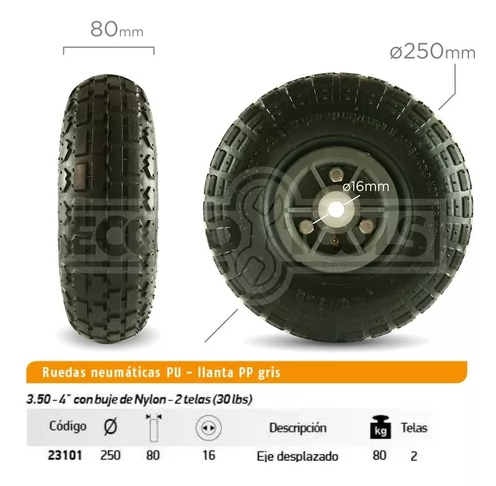
\includegraphics[width=.75\textwidth]{Figures/rueda.png}
\label{fig:rueda}
\caption{Datos de las ruedas elegidas}
\end{figure}

Al conocer el diámetro de las ruedas se pueden calcular el torque y las rpm de los motores.


\subsection{motores de tracción}

Para los motores de tracción de opto por motores PGM36-555, que son motores de 24V DC con reductor satelital, estos motores entregan 24Kgf/cm a 45rpm (58rpm en vacio) con un consumo de 0.7A, y un torque maximo de 80Kgf/cm con un consumo de 7.5A.

Con las ruedas previamente seleccionadas se puede calcular la velocidad robot

\begin{align*}
RPM &= 45 \\
D &= 0{,}25\,\text{m} \\
C &= \pi \cdot D = \pi \cdot 0{,}25 \approx 0{,}7854\,\text{m} \\
\end{align*}

Entonces la velocidad se calcula como:

\begin{align*}
v_{\text{m/s}} &= \frac{RPM \cdot C}{60} = \frac{45 \cdot 0{,}7854}{60} \approx 0{,}589\,\text{m/s} \approx 2{,}12\,\text{km/h}
\end{align*}

\subsection{Motores de la torreta}

Para los dos ejes de la torreta se opto por motores stepper por su capacidad de mantener la posición al mantener energizadas las bobinas.

Para el eje X se opto por un motor tipo nema 17 de aproximadamente 2.6Kg/cm de torque de holding.

Para el eje Y, ya que este tiene que sostener el peso del arma se opto por un motor tipo nema 23 con reductor tipo sinfin y corona.

\subsection{Drivers de motor}

Una vez definidos los motores se buscaron los drivers para estos.

Para los motores de traccion se seleccionaron modulos puente H basados en BTS7960 ya que soportan tenciones entre 5.5V y 27V y corrientes de hasta 43A.

Para el motor nema 17 del eje X se opto por el driver A4988

El motor nema 23 del eje Y ya poseia su propio driver TB6600

\subsection{Interfaz con la PC}

Como el procesamiento sera realizado en la pc y la interfaz solo cumple la tarea de traducir las ordenes de esta a los drivers de motor se opto por una placa de desarrollo arduino nano, ya que esta cuenta con un puerto serie para conectarse a la pc y suficientes pines I/O para controlar todos los motores necesarios.

\begin{figure}[H]
\centering
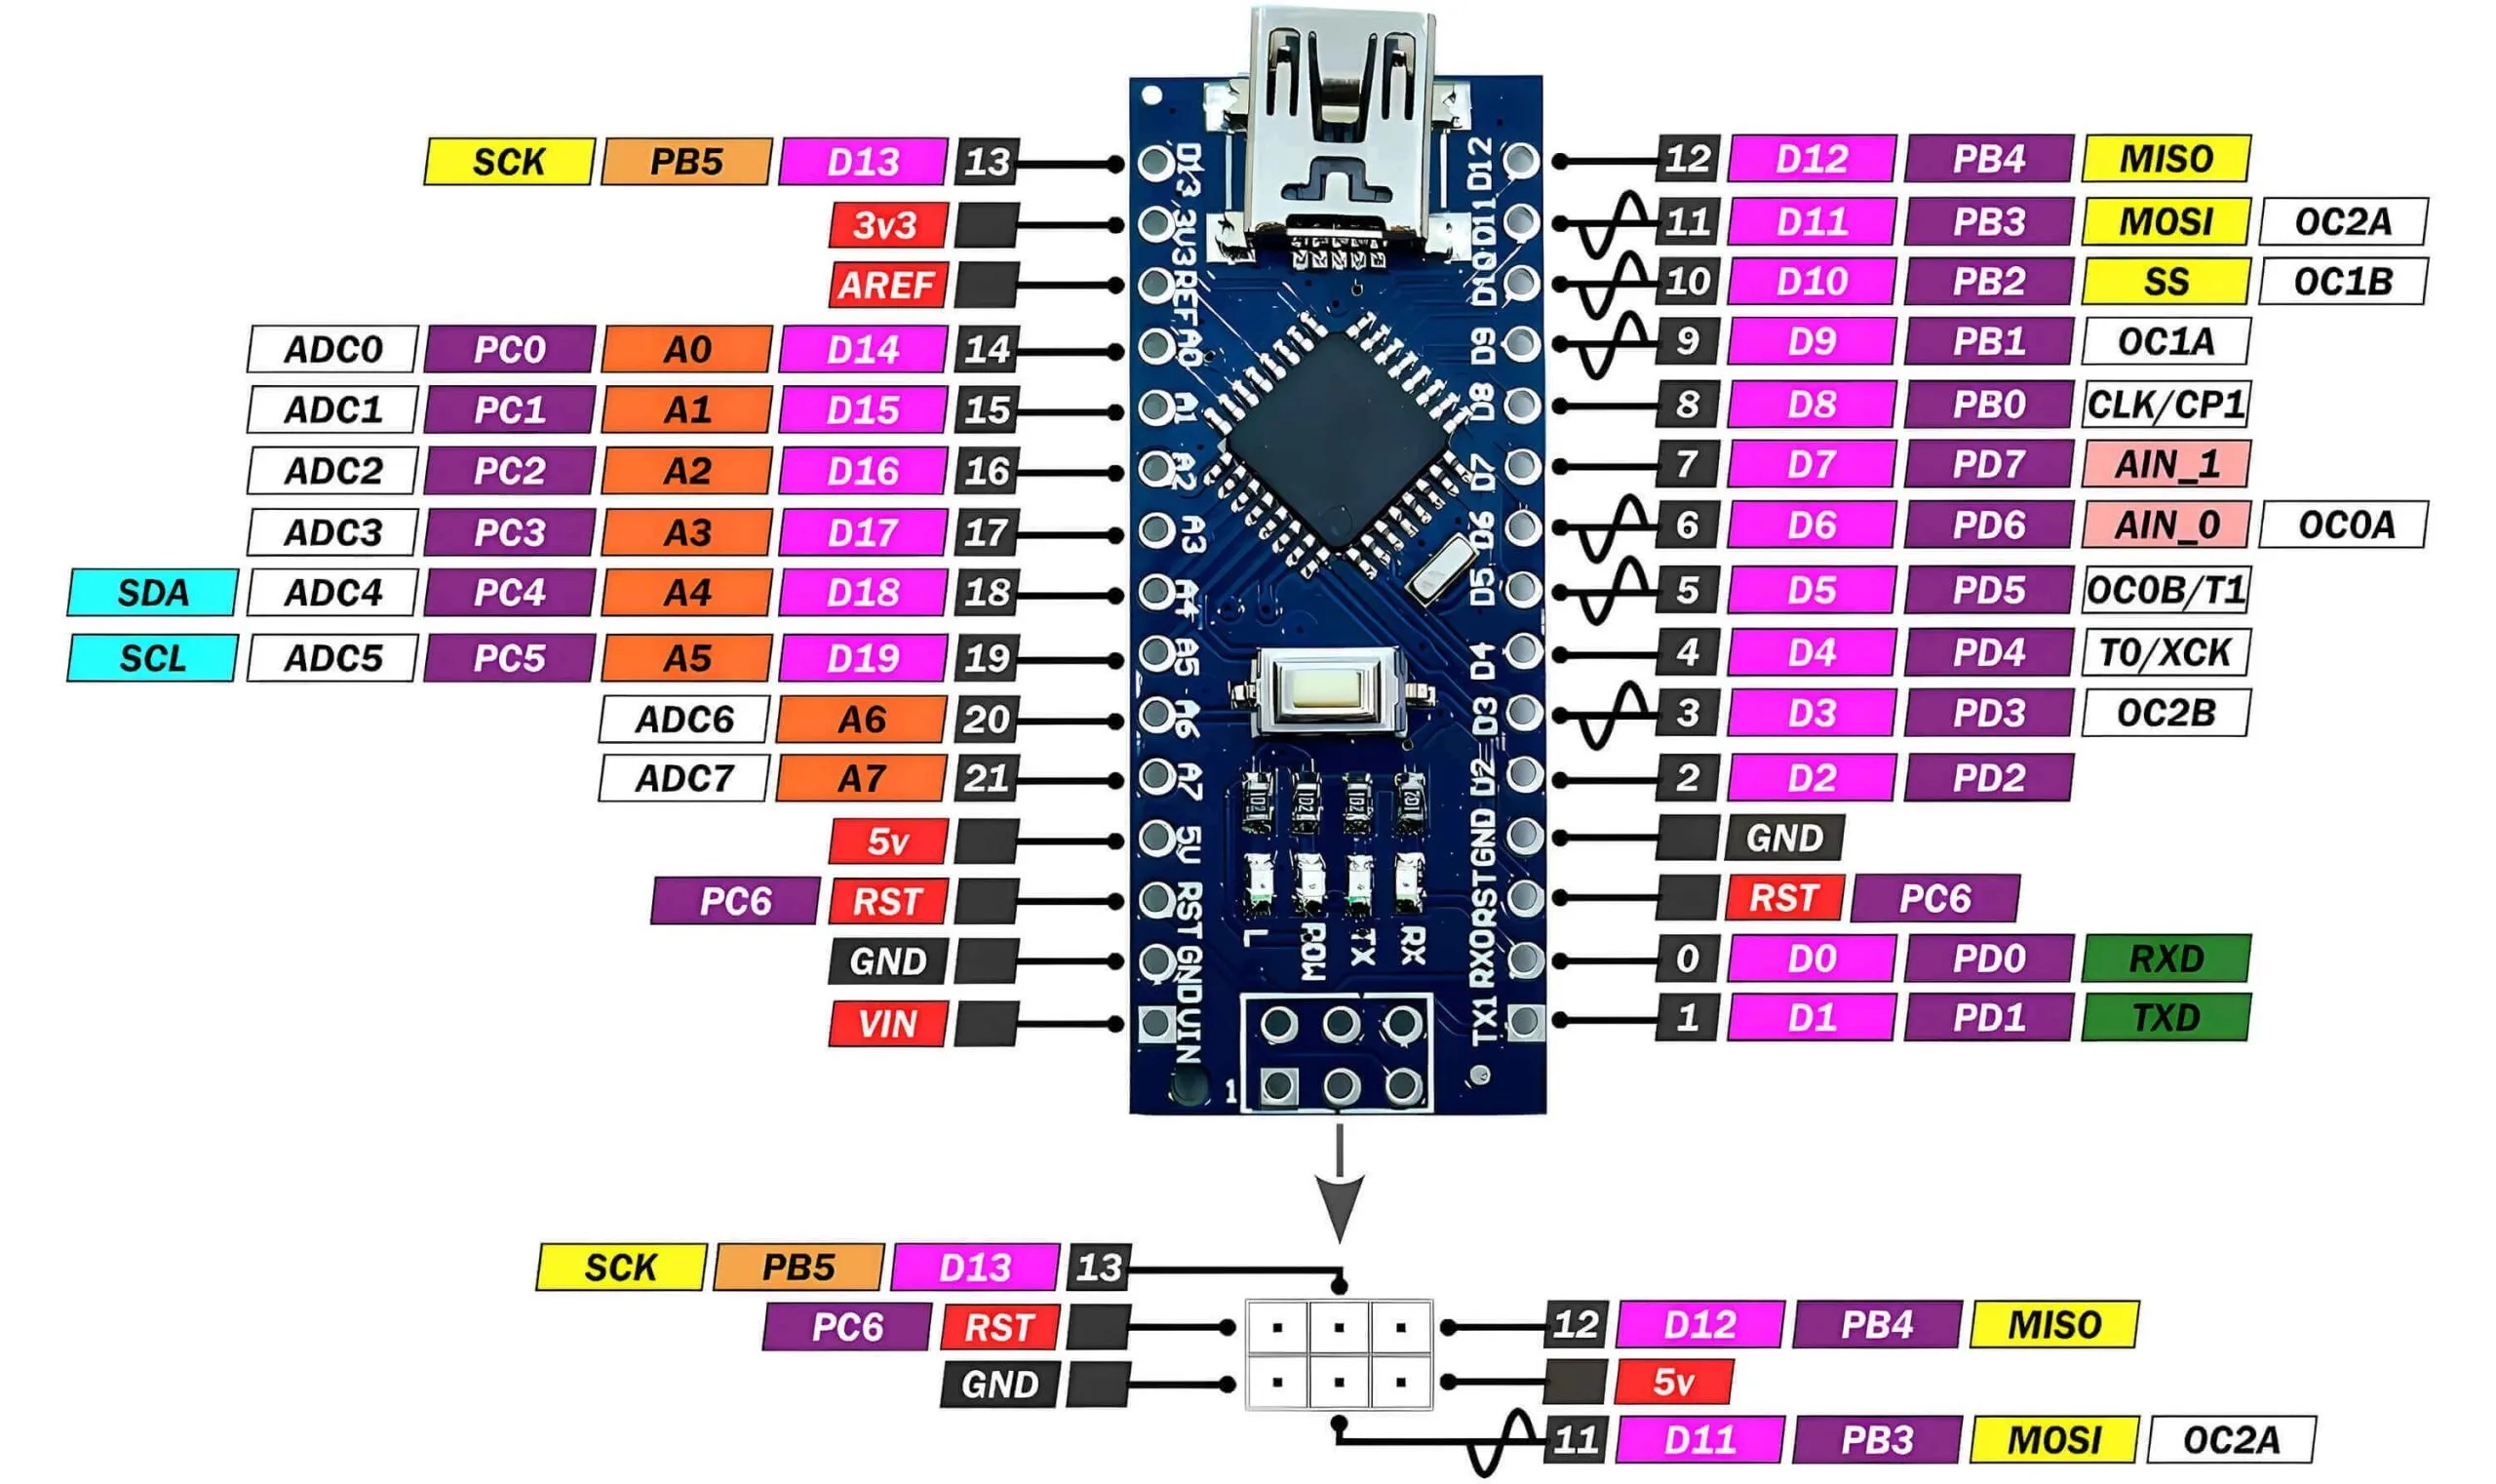
\includegraphics[width=1\textwidth]{Figures/arduino.jpg}
\label{fig:arduino}
\caption{Pinout del Arduino nano}
\end{figure}

\subsection{Baterias}

Ya que los motores serian alimentados a 24v se opto por usar baterias recargables de gel de 12V y 7Ah puestas en serie para obtener los 24V

\section{Chasis}
Para facilitar la fabricación se opto por un chasis impreso en 3D para la POC.

Durante el proceso de diseño se tuvieron en cuenta las particularidades del proceso de impresión y los limites de volumen de las impresoras disponibles.

Con el objetivo de utilizar solo dos motores y mantener el movimiento solidario de las ruedas por lado se opto por unir los ejes delantero y trasero de cada lado con cadenas.

El diseño del chasis del robot se puede subdividir en secciones básicas que se unen entre si:

\begin{itemize}
    \item \textbf{Ejes:} Soportan el peso del robot y transmiten la energía a las ruedas.

    \item \textbf{Largueros del chasis:} Proporcionan rigidez y junto con los ejes forman las unidades básicas de tracción del robot.

    \item \textbf{Pisos:} Terminan de conformar la base y proporcionan el lugar para almacenar baterías y la electrónica.

    \item \textbf{Coraza superior:} Da soporte a los componentes externos y la torreta. 

    \item \textbf{Torreta:} Da soporte y permite apuntar el arma, telémetro y la cámara principal. 

\end{itemize}

\subsection{Análisis de Implementación}

A continuación, se presenta un análisis detallado de las secciones básicas del chasis del robot y su implementación


\subsubsection{Ejes}

Los ejes tienen que soportar el peso del robot y al mismo tiempo transmitir la rotacion de los motores a las ruedas traseras y delanteras de cada lado de manera solidaria. Por esta razon se decidieron usar dos rulemanes de apoyo para soportar el peso de manera mas estable y se decidio agregar un piñon para unir las ruedas delanteras y traseras de cada lado con una cadena.

La estructura se compone de un eje central de metal, con los alojamientos para los dos rulemanes de apoyo, el piñón y el plato que sostiene la llanta, el cual tiene una chaveta para evitar que gire.

Los motores de tracción se fijan a los ejes con prisioneros que traban en el biselado de los ejes de los motores.

\begin{figure}[H]
\centering
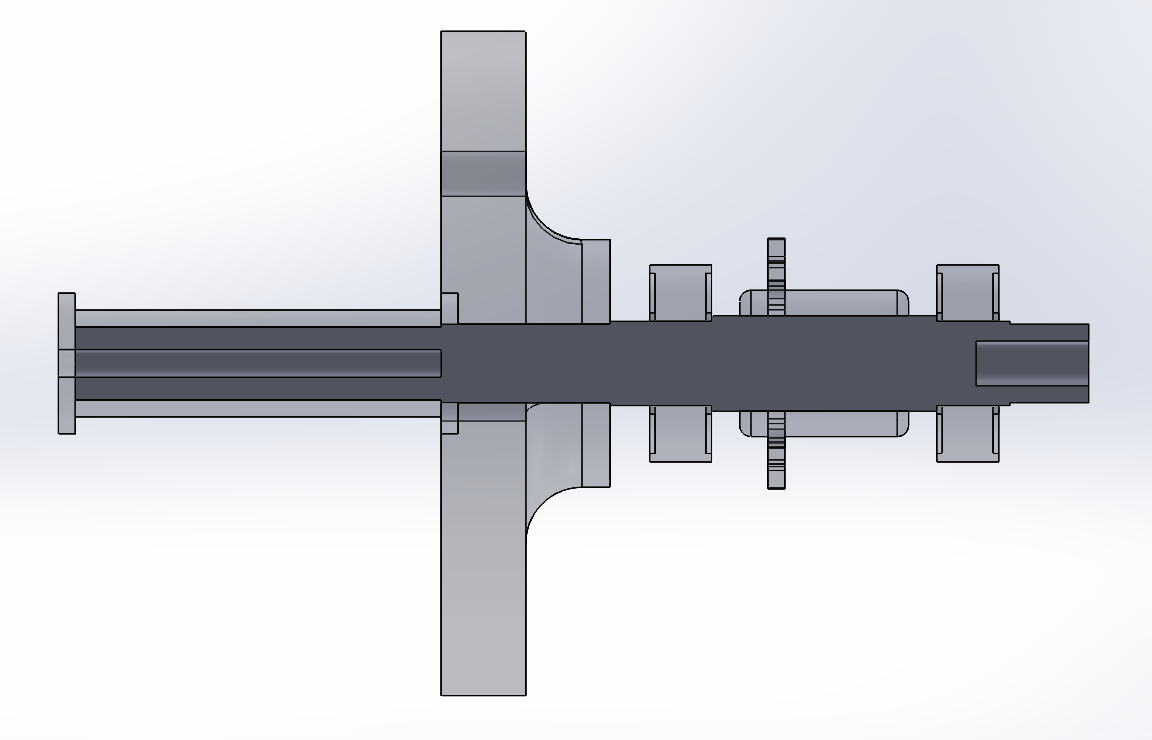
\includegraphics[width=1\textwidth]{Figures/eje_corte.png}
\label{fig:eje}
\caption{Corte del eje}
\end{figure}

\subsubsection{Largueros del chasis}

Los encargados de dar soporte a los ejes y mantener las cadenas de transmisión en su lugar son los largueros del chasis, los cuales son las piezas centrales en la estructura de la plataforma y junto con los motores y ruedas forman las unidades básicas de tracción del robot.

Se componen de 7 secciones, de las cuales 6 son la estructura del larguero y una ultima el soporte para el motor de tracción. En caso de cambiar a un esquema de 4 motores de tracción solamente es necesario agregar una placa de soporte extra delante ya que el diseño es simétrico.

Estas piezas deben ser ensambladas alrededor de los ejes de tracción ya que también limitan el movimiento axial de los rulemanes.

\begin{figure}[H]
\centering
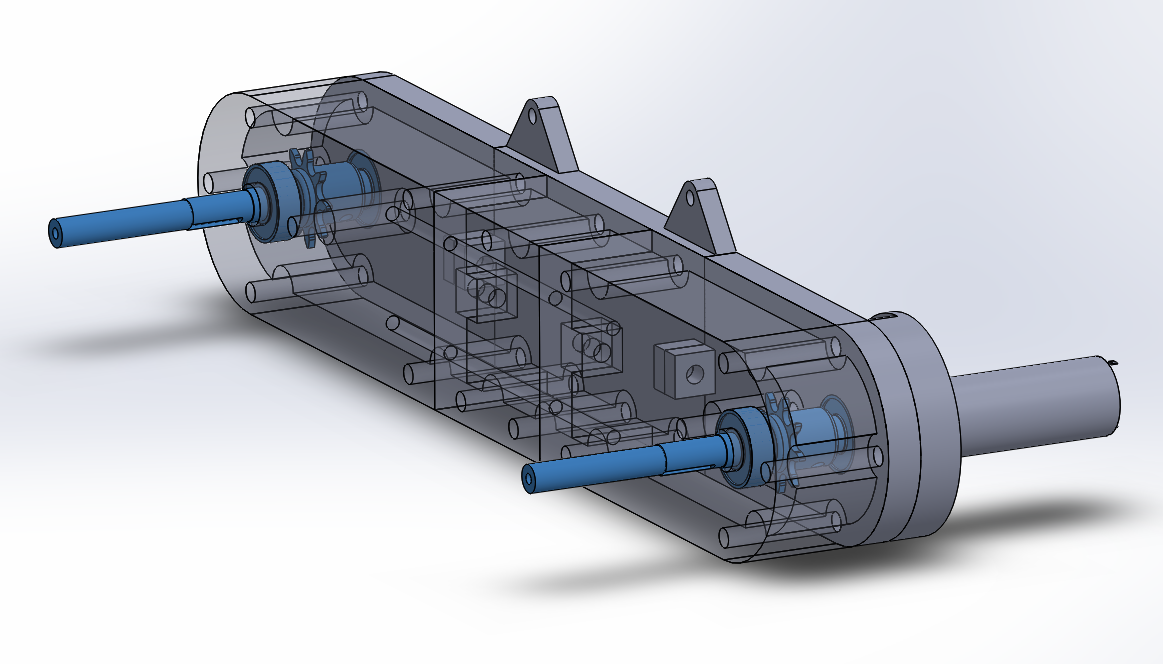
\includegraphics[width=1\textwidth]{Figures/larguero.png}
\label{fig:base}
\caption{Largueros del chasis}
\end{figure}

\subsubsection{Pisos}

Los pisos se agregan a los largueros para terminar de conformar la estructura de la plataforma, la cual esta diseñada por secciones imprimibles que luego se unen entre si con varillas transversales para dar rigidez y fuerza al conjunto.

\begin{figure}[H]
\centering
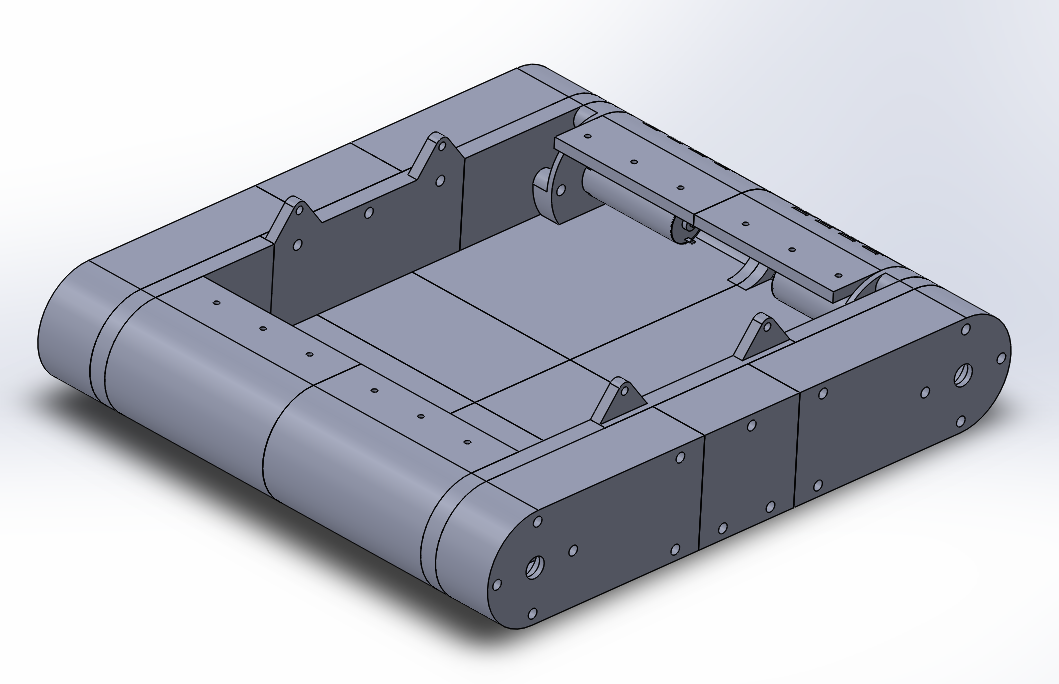
\includegraphics[width=1\textwidth]{Figures/base_sola.png}
\label{fig:base}
\caption{Base del robot}
\end{figure}

\subsubsection{Coraza superior}

La coraza superior se diseño con forma de caparazón angulado, con una apertura para el sensor LIDAR y una plataforma para llevar la PC (que para simplificar las pruebas se dejo afuera del prototipo).

En el diseño de la coraza también se busco solucionar la limitación en el volumen de impresión por lo que se diseño una estructura con piezas que se intercalan para obtener rigidez, lo cual es esencial ya que la coraza da soporte a la torreta principal.

\begin{figure}[H]
\centering
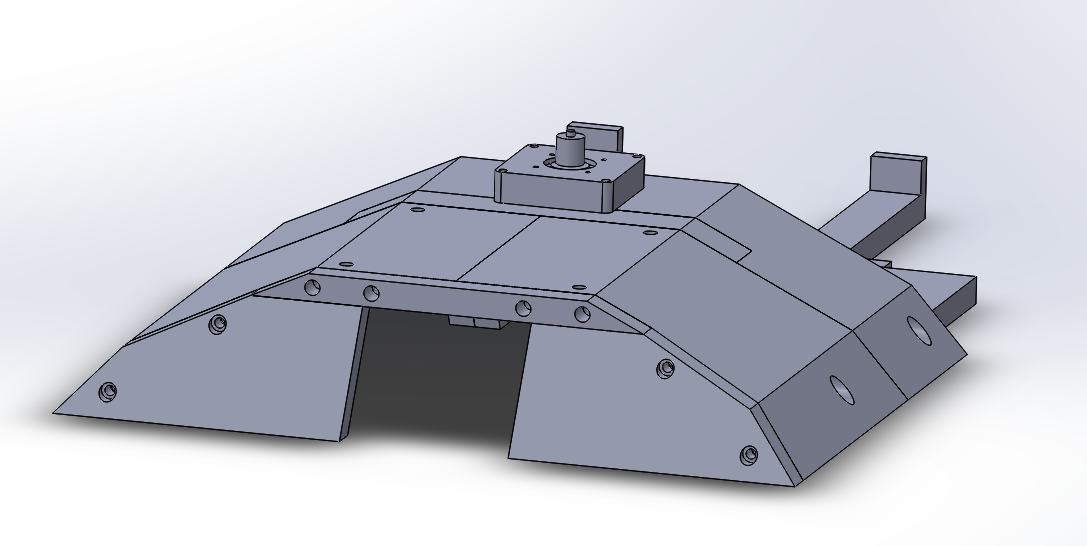
\includegraphics[width=1\textwidth]{Figures/coraza sola.png}
\label{fig:base}
\caption{Coraza superior}
\end{figure}

\subsubsection{Torreta}

La torreta se compone de una plataforma giratoria para el eje X que se conecta al motor con una correa y sobre esta plataforma se monto el soporte del motor y el arma con la articulación del eje Y.

El arma se agarra de un aplique fijo en su riel, en posición invertida.

\begin{figure}[H]
\centering
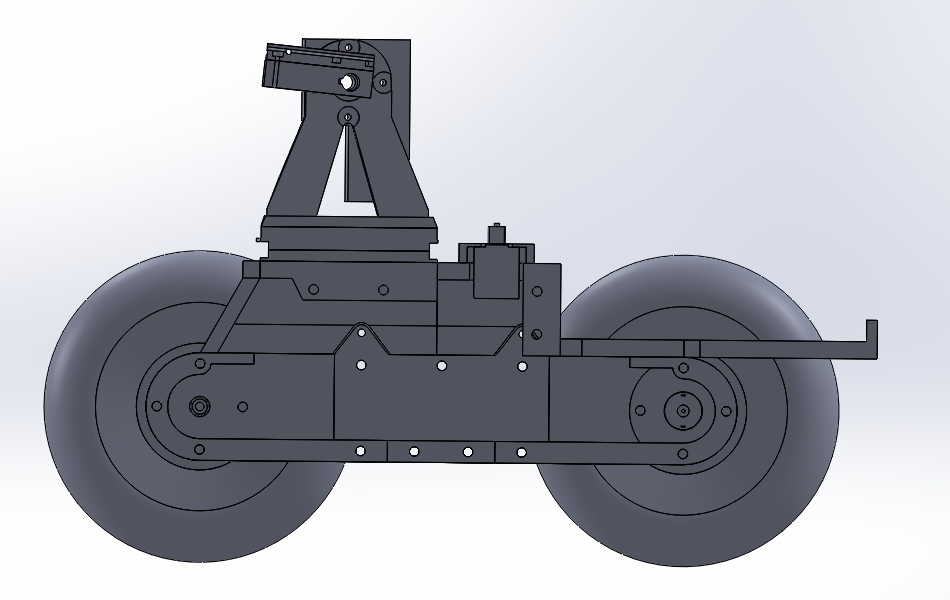
\includegraphics[width=1\textwidth]{Figures/corte robot.png}
\label{fig:robot}
\caption{Corte lateral del robot}
\end{figure}

\subsubsection{Ensamblaje completo}

Las partes superior e inferior de la coraza se ensamblan con 4 encastres triangulares, lo cuales adicionalmente se aseguran con 4 tornillos y se conforma entonces la estructura completa del chasis del prototipo.

\begin{figure}[H]
\centering
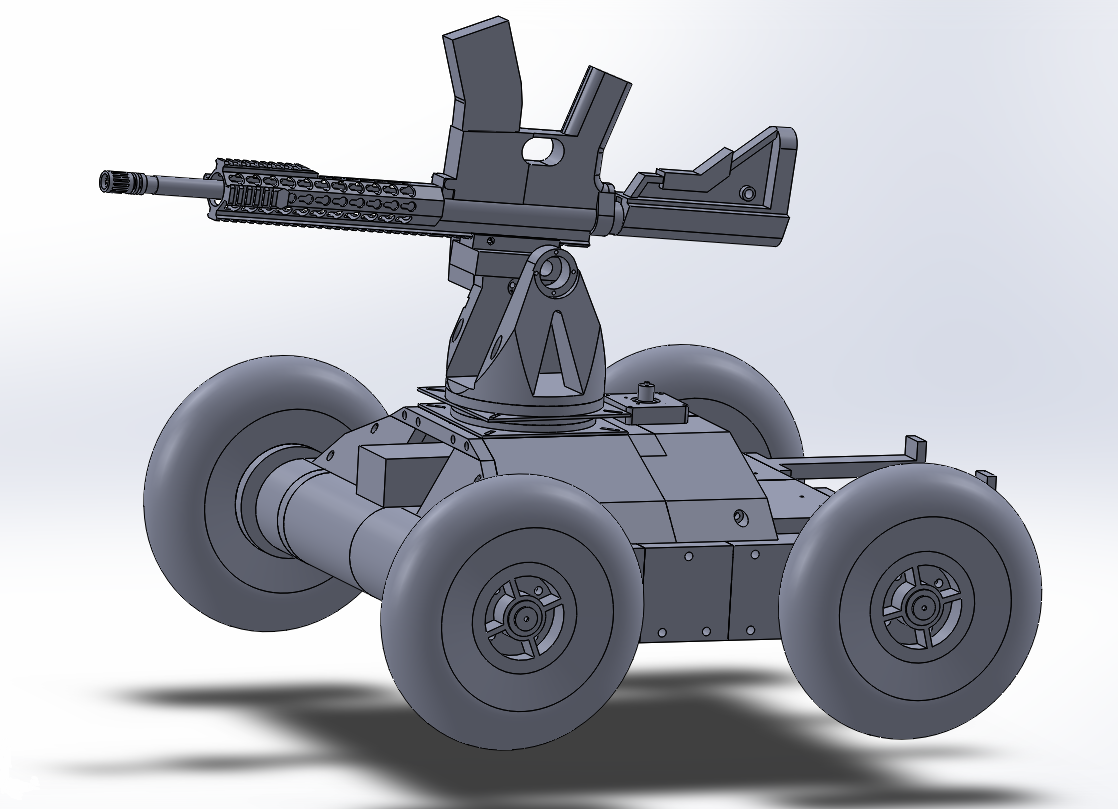
\includegraphics[width=1\textwidth]{Figures/robot_completo.png}
\label{fig:robot}
\caption{Robot completo}
\end{figure}

Para reducir tiempos y costos de prototipado se simularon por computadora las interacciones entre las piezas y la funcionalidad del prototipo lo que permitió que todas las partes funcionaran correctamente juntas antes de comenzar la impresión.

\subsection{Conclusiones del Análisis de Implementación}

El diseño del chasis se centro en los objetivos planteados para esta POC, se priorizo la facilidad de fabricación mediante impresión 3D y aseguro la modularidad y funcionalidad mecánica necesarias para el desplazamiento y operación del robot.

La estructura modular, segmentada en ejes, largueros, pisos, coraza y torreta, facilitó tanto el ensamblaje como la adaptación a cambios de diseño futuros.

Asimismo, se logró una integración estructural eficiente entre las piezas impresas, y un diseño que considera las limitaciones del volumen de impresión y maximiza la rigidez del conjunto. La simulación previa al prototipado físico permitió validar ensamblajes y detectar interferencias o problemas potenciales, y de esta manera reducir tiempos y costos en la fase de fabricación.
\section{Software}

El desarrollo del software del robot militar se realizó siguiendo el paradigma de Programación Orientada a Objetos (POO), permitiendo una estructura modular y escalable. Esta arquitectura facilita la separación clara de responsabilidades, el mantenimiento del código y la posibilidad de extender funcionalidades sin afectar el comportamiento general del sistema.

El sistema está dividido en tres módulos principales: control de misión, navegación autónoma y seguimiento de objetivos. Cada uno de estos módulos interactúa a través de interfaces bien definidas, lo que permite la sustitución o mejora de componentes sin necesidad de modificar el resto del sistema.

\begin{itemize}
    \item \textbf{Control de misión:} Administra el estado general del robot y coordina los distintos subsistemas según el tipo de misión. Incluye lógica para transiciones entre estados como patrullaje, búsqueda de objetivos, eliminación y navegación hacia puntos estratégicos. También gestiona el tiempo de ejecución y las condiciones de activación de cada misión.

    \item \textbf{Seguimiento de objetivos:} Utiliza técnicas de visión computacional para analizar imágenes recibidas en tiempo real y detectar objetivos. Emplea controladores PID para alinear la torreta del robot con el objetivo detectado y evalúa condiciones de disparo según el nivel de precisión alcanzado.

    \item \textbf{Navegación autónoma:} Se basa en mapas de ocupación del entorno y algoritmos de planificación de trayectorias para determinar rutas seguras hacia los puntos de interés. Este módulo considera tanto la posición como la orientación del robot, y ajusta los comandos de movimiento para alcanzar los objetivos de forma precisa y eficiente.

    \item \textbf{Interfaces modulares:} El sistema fue diseñado para funcionar tanto en un entorno simulado como en uno real. Para ello, se implementaron drivers abstractos que permiten controlar el robot mediante simuladores (como gamepads virtuales) o hardware real sin alterar la lógica del sistema principal. De igual manera, la comunicación entre módulos se realiza mediante un sistema de colas de mensajes, que asegura una interacción desacoplada y eficiente entre procesos.

\end{itemize}

Gracias a esta estructura modular y orientada a objetos, el software no solo puede adaptarse a distintos escenarios operativos, sino que también facilita futuras mejoras, pruebas automatizadas y escalabilidad hacia sistemas más complejos o entornos reales de combate.

\subsection{Máquina de Estados Finitos}

El comportamiento general del robot se organiza como una máquina de estados finitos (FSM, por sus siglas en inglés), lo que permite una lógica de control clara, robusta y fácilmente extensible. Cada estado representa una configuración operativa particular del robot, y las transiciones entre ellos se determinan en función de eventos y condiciones específicas del entorno o de la misión.

\subsubsection{Estados Principales}

\begin{itemize}
    \item \textbf{STARTING:} Estado inicial del sistema. Evalúa el tipo de misión configurada y decide si comenzar en modo \texttt{SENTINEL} o \texttt{NAVIGATING}.

    \item \textbf{SENTINEL:} Modo de vigilancia estática en el que el robot escanea el entorno en busca de objetivos utilizando visión computacional. Si se detecta un objetivo, se transiciona al estado \texttt{TRACKING}.

    \item \textbf{TRACKING:} El robot ajusta la orientación de su torreta para seguir un objetivo en movimiento. Si logra un seguimiento preciso, transiciona al estado \texttt{TRACK\_N\_KILL}. Si pierde el objetivo, regresa a \texttt{SENTINEL} o \texttt{NAVIGATING}, dependiendo del estado anterior interrumpido.

    \item \textbf{TRACK\_N\_KILL:} Estado en el cual el robot ha fijado un blanco con alta precisión y activa su mecanismo de ataque. Si se pierde la fijación, vuelve a \texttt{TRACKING}.

    \item \textbf{NAVIGATING:} Estado de navegación autónoma hacia puntos estratégicos definidos en la misión. Si se detecta un objetivo durante la marcha, el sistema cambia a \texttt{TRACKING}. Al alcanzar un objetivo con tipo de misión de vigilancia, cambia a \texttt{SENTINEL}.

    \item \textbf{IDLE / PATROLLING / MAPPING:} Estados secundarios que permiten al robot detenerse, patrullar o explorar el entorno. Aunque no fueron parte del flujo principal en el prototipo básico, están contemplados para futuras funcionalidades.

    \item \textbf{DEBUG / ERROR:} Estados especiales para depuración o manejo de fallas críticas en tiempo de ejecución.
\end{itemize}

\subsection*{Transiciones}

Las transiciones entre estados se determinan mediante condiciones lógicas evaluadas en tiempo real:

\begin{itemize}
    \item \textbf{STARTING $\rightarrow$ SENTINEL/NAVIGATING:} Según si la misión es de vigilancia estática o de desplazamiento.
    \item \textbf{SENTINEL $\rightarrow$ TRACKING:} Activada cuando el sistema de visión detecta un objetivo.
    \item \textbf{TRACKING $\rightarrow$ TRACK\_N\_KILL:} Cuando el objetivo está centrado y estable.
    \item \textbf{TRACKING $\rightarrow$ SENTINEL/NAVIGATING:} Si se pierde el objetivo, se regresa al estado anterior.
    \item \textbf{TRACK\_N\_KILL $\rightarrow$ TRACKING:} Si se pierde la fijación sobre el objetivo.
    \item \textbf{NAVIGATING $\rightarrow$ TRACKING:} Si se detecta un objetivo durante el trayecto.
    \item \textbf{NAVIGATING $\rightarrow$ SENTINEL:} Cuando se alcanza el destino y el tipo de misión lo requiere.
\end{itemize}

Este enfoque basado en FSM proporciona una estructura robusta y predecible para la toma de decisiones del robot, facilitando además su validación mediante pruebas controladas y su extensión hacia escenarios más complejos.

\begin{figure}[htbp]
\centering
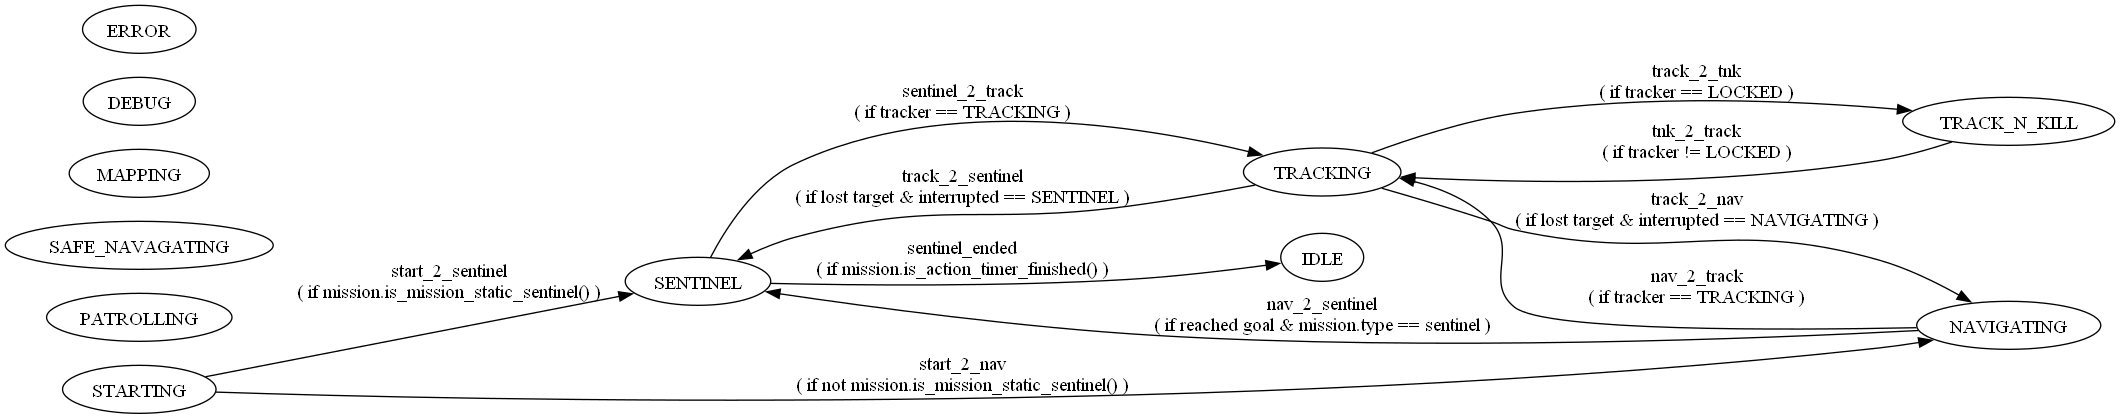
\includegraphics[width=.99\textwidth]{Figures/maquina_de_estados.png}
\label{fig:Maquina_de_estado}
\caption{Máquina de estados finitos del prototipo}
\end{figure}

\subsection{Análisis de Implementación}

A continuación, se presenta un análisis detallado de la implementación del sistema, organizado en subsecciones que corresponden a los componentes clave del software. Este análisis se centra en el funcionamiento y el rol de cada componente dentro del sistema global, destacando los aspectos teóricos y las decisiones de diseño que sustentan su desarrollo. Cuando es relevante, se incluyen fragmentos de código para ilustrar conceptos específicos.

\subsubsection{Control Central y Coordinación de Módulos}

El componente central de control actúa como el núcleo del sistema robótico, encargado de coordinar las interacciones entre los módulos de seguimiento de objetivos y navegación autónoma, además de gestionar las transiciones de estado según la máquina de estados finitos descrita. Su rol principal es asegurar que el robot opere de manera coherente, alternando entre diferentes comportamientos según las condiciones de la misión y los eventos del entorno.

Desde un punto de vista teórico, este componente implementa un patrón de diseño de \textit{mediador}, donde un elemento central coordina las interacciones entre múltiples subsistemas sin que estos se comuniquen directamente entre sí. Esto reduce el acoplamiento y mejora la modularidad, ya que los módulos solo interactúan con el controlador central a través de interfaces bien definidas. Además, la capacidad de inicializar diferentes tipos de controladores para hardware virtual o real refleja el principio de \textit{inversión de dependencias}, permitiendo que el sistema sea independiente de la implementación específica del hardware.

El bucle principal del sistema actualiza continuamente la posición y orientación del robot mediante mensajes recibidos de un sistema de colas de mensajería. Este enfoque de procesamiento basado en eventos es típico en sistemas reactivos, donde el robot debe responder en tiempo real a cambios en el entorno o a nuevas detecciones de objetivos. Un aspecto crítico del diseño es la gestión de interrupciones, como cuando se detecta un objetivo durante la navegación. El sistema guarda el estado anterior para permitir la reanudación de la tarea original una vez que se pierde el objetivo, lo que demuestra un manejo robusto de prioridades en un entorno dinámico.

\subsubsection{Seguimiento de Objetivos y Control de Torreta}

El módulo de seguimiento de objetivos es responsable de detectar y seguir objetivos mediante visión computacional, así como de controlar la torreta del robot para alinearla con el objetivo detectado. Su rol es crucial en las fases de vigilancia y ataque, permitiendo al robot identificar amenazas y actuar en consecuencia.


Este módulo utiliza un controlador PI (Proporcional-Integral), que combina términos proporcional e integral para minimizar el error entre la posición deseada y la actual de la torreta. Se optó por no incluir el término derivativo debido a que puede amplificar el ruido presente en las mediciones de la cámara y causar movimientos erráticos de la torreta. En la implementación, se observa cómo se limitan los valores integrales y de salida para evitar comportamientos inestables, como oscilaciones excesivas. A continuación, se muestra un fragmento de código que ilustra este control PI:

\begin{lstlisting}[language=Python, caption=Control PI para seguimiento de objetivos, label=lst:control_pi]
# Detectar objetivo en la imagen
objetivo = detectar_objetivo(imagen_camara)

# Calcular error de posicion respecto al centro
error_actual = calcular_error(objetivo, centro_pantalla)

# Aplicar control PI (sin termino derivativo)
error_proporcional = error_actual
error_integral += error_actual
salida_pi = Kp * error_proporcional + Ki * error_integral

# Limitar salida para evitar oscilaciones
salida_limitada = limitar_salida(salida_pi)

# Ajustar orientacion de la torreta
torreta.mover(salida_limitada)

# Si el objetivo esta centrado, activar disparo
if objetivo_centrado(error_actual):
    sistema_disparo.activar()
\end{lstlisting}
El módulo procesa datos de video recibidos a través de un sistema de mensajería, filtrando objetivos según una etiqueta específica y calculando el centro del cuadro delimitador del objetivo con mayor confianza. Luego, determina si el objetivo está dentro de un margen de seguridad para decidir si está en modo de bloqueo (listo para disparar) o de seguimiento activo. Este enfoque de umbral binario simplifica la decisión de disparo, aunque podría mejorarse con técnicas más avanzadas como filtros de Kalman para suavizar las trayectorias de seguimiento.

Además, cuando no hay objetivos detectados, el módulo implementa un comportamiento de búsqueda, moviendo la torreta en un patrón de barrido definido por ángulos máximos y mínimos. Este comportamiento refleja un enfoque de exploración sistemática, común en sistemas de vigilancia autónoma.

\subsubsection{Navegación Autónoma y Planificación de Rutas}

El módulo de navegación autónoma gestiona el desplazamiento del robot hacia puntos de interés definidos en una misión. Su rol es determinar rutas seguras y eficientes utilizando mapas de ocupación del entorno y algoritmos de planificación de trayectorias, asegurando que el robot alcance sus objetivos mientras evita obstáculos.

Desde una perspectiva teórica, la navegación autónoma integra localización, mapeo y planificación de rutas. Este módulo calcula rutas óptimas mediante el algoritmo A*, como se discutió en la sección teórica previa. Carga un mapa de ocupación y genera una ruta hacia el objetivo, almacenando los puntos intermedios (waypoints) para su seguimiento. El control de movimiento ajusta la velocidad lineal y angular del robot en función de la distancia y el ángulo hacia el objetivo, utilizando un enfoque proporcional simple para evitar sobrepasar el destino, como se muestra en el siguiente fragmento:

\begin{lstlisting}[language=Python, caption=Control proporcional para navegación, label=lst:control_proporcional]
# Calcular distancia al objetivo
distancia_al_objetivo = calcular_distancia(posicion_actual, objetivo)

# Control proporcional de velocidad
velocidad_adelante = distancia_al_objetivo * ganancia_velocidad
velocidad_adelante = limitar_velocidad(velocidad_adelante)

# Calcular error angular y ajustar giro
error_angular = calcular_error_orientacion(objetivo)
velocidad_giro = error_angular * ganancia_giro
velocidad_giro = limitar_giro(velocidad_giro)

# Mover el robot
robot.mover(velocidad_adelante, velocidad_giro)
\end{lstlisting}

Este método podría beneficiarse de controladores más sofisticados como PID o MPC (Model Predictive Control) para manejar dinámicas más complejas o terrenos irregulares. Un aspecto notable es el registro de la trayectoria del robot, que se guarda para análisis posterior y depuración, un aspecto crucial en el desarrollo de sistemas autónomos.

\subsubsection{Comunicación y Mensajería entre Módulos}

El sistema de comunicación basado en colas de mensajes es fundamental para la arquitectura desacoplada del software, permitiendo que los módulos intercambien datos como imágenes procesadas o información de posición sin una conexión directa. Su rol es asegurar una interacción eficiente y asíncrona entre los componentes del sistema.

Teóricamente, este sistema implementa el patrón de diseño \textit{publish-subscribe} combinado con colas de trabajo, lo que asegura que los mensajes sean persistentes y procesados de manera ordenada. Permite a los módulos acceder a los datos más recientes o limpiar la cola para evitar acumulación de mensajes obsoletos, lo que es crítico en aplicaciones en tiempo real donde la latencia debe minimizarse. Este enfoque de comunicación asíncrona es ideal para sistemas distribuidos, ya que permite que los componentes operen de manera independiente y a diferentes velocidades de procesamiento. Sin embargo, introduce desafíos como la gestión de errores en la decodificación de mensajes y la posible pérdida de datos si no se implementan mecanismos de confirmación adecuados.

\subsubsection{Configuración y Modularidad del Sistema}

Un tema recurrente en la implementación es el uso de archivos de configuración para parametrizar el comportamiento del sistema. Esto se observa en la inicialización de todos los módulos principales, donde parámetros como ganancias de control, márgenes de seguridad y configuraciones de hardware se cargan dinámicamente. Desde un punto de vista teórico, este enfoque sigue el principio de \textit{configuración sobre convención}, permitiendo ajustes sin modificar la lógica interna, lo que es esencial para pruebas y adaptaciones a diferentes entornos o hardware.

Además, la modularidad se refuerza mediante el uso de controladores virtuales que abstraen la interacción con el hardware. Esto refleja el patrón de diseño \textit{adaptador}, facilitando la transición entre simulación y operación real, un aspecto clave en el desarrollo de sistemas robóticos donde las pruebas en hardware físico pueden ser costosas o peligrosas.

\subsection{Conclusiones del Análisis de Implementación}

El análisis de la implementación revela un diseño de software bien estructurado, basado en principios de modularidad, desacoplamiento y configurabilidad. La implementación de una máquina de estados finitos proporciona un marco robusto para la toma de decisiones, mientras que los módulos de seguimiento y navegación utilizan técnicas de control clásicas y modernas para cumplir con los objetivos de la misión. El sistema de comunicación asegura una interacción eficiente entre componentes, aunque podría beneficiarse de mecanismos adicionales de manejo de errores y sincronización.

En términos teóricos, el software refleja una combinación de enfoques reactivos y deliberativos: reactivos en la respuesta inmediata a detecciones de objetivos, y deliberativos en la planificación de rutas y gestión de misiones. Esta dualidad es típica en robótica autónoma, donde se requiere un equilibrio entre rapidez de respuesta y planificación a largo plazo. Futuras mejoras podrían incluir la integración de algoritmos de aprendizaje automático para la adaptación dinámica de parámetros de control y la implementación de técnicas de fusión de sensores para mejorar la robustez en entornos complejos.
\section{Interfaz y control de motores}

El desarrollo de la interfaz entre la PC y los motores del robot se realizó priorizando funcionalidad, simplicidad y robustez. El sistema se diseñó para que la placa controladora actúe únicamente como una unidad de control de bajo nivel, recibiendo comandos desde la PC y ejecutando las órdenes directamente sobre los actuadores, sin necesidad de procesamiento complejo en el microcontrolador.

Este diseño modular permite además implementar distintos modos de operación sin modificar el hardware: control local desde una computadora de abordo, teleoperación remota o integración con sistemas autónomos, cambiando únicamente el medio físico de comunicación.

\subsection{Análisis de Implementación}
El sistema de control está dividido en tres capas software principales:

\begin{itemize}
    \item \textbf{Capa de aplicación (PC):}
Utiliza la clase RobotDriver, que actúa como interfaz de alto nivel (wrapper) para generar comandos de movimiento, torreta y disparo sin interactuar directamente con los frames del protocolo.

    \item \textbf{Capa de comunicación (PC–Microcontrolador):}  
Implementada en la PC en Python mediante RobotConnector, encargada de formar, enviar y validar tramas sobre el enlace UART. Y en el Microcontrolador en C++ mediante RobotListener, encargade de recepción, decodificación y validación de tramas.

    \item \textbf{Capa de control de hardware (Microcontrolador):}
Implementa la clase Robot, encargada del control directo de motores DC, motores paso a paso e IO mediante interrupciones.
\end{itemize}


Dentro de la implementacion las partes mas destacables son la capa de comunicacion y la de control de hardware.

\subsubsection{Comunicacion}

La comunicación entre la PC y la placa se implementó sobre un enlace UART, utilizando un protocolo propio basado en tramas compactas de longitud variable.

\begin{figure}[H]
\centering
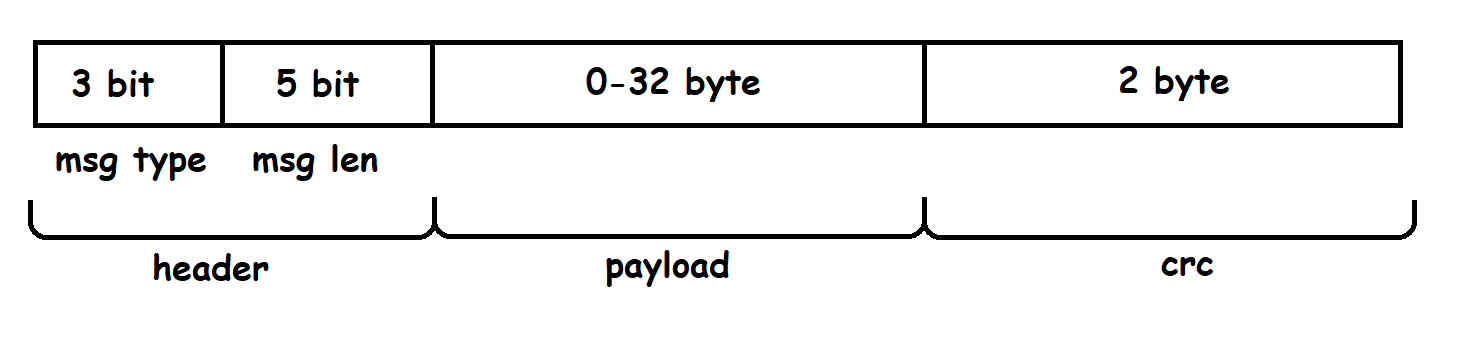
\includegraphics[width=.99\textwidth]{Figures/protocolo.png}
\label{fig:Trama}
\caption{Trama del protocolo}
\end{figure}


\begin{table}[h]
\centering
\begin{tabular}{l l l p{6cm}}
\toprule
\textbf{Tipo} & \textbf{Código} & \textbf{Payload} & \textbf{Uso} \\
\midrule
ping    & 0b000 & No       & Verificación de enlace. \\
data    & 0b001 & Sí       & Envio de data. \\
angle   & 0b010 & No       & Consulta de posición de la torreta. \\
ack     & 0b011 & No       & Confirmación válida. \\
nak     & 0b100 & No       & Error de CRC, solicitar retransmisión. \\
home    & 0b101 & No       & Enviar torreta a origen. \\
metrics & 0b110 & No       & Solicita datos del sistema. \\
stop    & 0b111 & No       & Detener actuadores. \\
\bottomrule
\end{tabular}
\caption{Mensajes, códigos y uso del payload}
\end{table}

El flujo completo de comunicación es el siguiente:

\begin{enumerate}
    \item \textbf{Generación de la trama en la PC:}  
    Se construye la trama, incluyendo el encabezado, el payload y el CRC-16 correspondiente.

    \item \textbf{Transmisión hacia el microcontrolador:}  
    La trama completa se envía.

    \item \textbf{Recepción y decodificación en la placa:}  
    El microcontrolador recibe los bytes, interpreta el encabezado y separa el payload y el CRC recibido.

    \item \textbf{Validación mediante CRC:}  
    La placa calcula localmente el CRC-16 del header y payload recibidos y lo compara con el CRC transmitido:
    \begin{itemize}
        \item Si los valores \textbf{coinciden}, la trama es válida:  
        la placa ejecuta el comando solicitado y responde con una trama de tipo \texttt{ACK}.
        \item Si los valores \textbf{no coinciden}, se considera error de transmisión:  
        la placa responde con una trama \texttt{NAK}.
    \end{itemize}

    \item \textbf{Retransmisión automática en caso de error:}  
    Si la PC recibe un \texttt{NAK}, interpreta que ocurrió un error de comunicación y retransmite automáticamente la última trama enviada, garantizando la entrega confiable del comando.

    \item \textbf{Pedido de datos de telemetria:}  
    Si el controlador recibe un frame de tipo \texttt{metrics}, entonces responde con una trama de tipo \texttt{data} con la información de las métricas, la respuesta de tipo \texttt{data} se interpreta como un \texttt{ACK}.
\end{enumerate}
El CRC utilizado es CRC-16 con polinomio \texttt{0x1021} e inicialización \texttt{0xFFFF}, calculado sobre el header y el payload. 

Ademas se implementa un timeout para la recepción de la confirmación, de esta manera se asegura un funcionamiento robusto del sistema incluso en presencia de ruido o pérdidas temporales en el enlace.


Para controlar el robot se usan principalmente tramas de tipo \texttt{data} compuestas de la siguiente manera:

\texttt{[0b001101][velL, velR, velPitch, velYaw, shoot][CRC]}


Las velocidades estan expresadas entre 0 y 255, siendo 0 velocidad totalmente negativa, 255 maxima velocidad positiva y 128 velocidad 0.

\subsubsection{Drivers}
Para el control del robot se utilizaron dos tipos de actuadores:
\begin{itemize}
    \item Motores DC con puente H, utilizados para tracción.

    \item Motores paso a paso, utilizados para la torreta.
\end{itemize}
Debido a las diferencias entre ambos actuadores, los controladores fueron diseñados de forma independiente.
\subsubsection{Drivers para motor de tracción}
Los puentes H que usan los motores de tracción izquierdo y derecho son controlados mediante tres señales, dos de dirección que controlan el sentido de giro y una de marcha en la que se utiliza PWM benedictino un control de la velocidad de giro de las ruedas.

Para las señales PWM se utilizo el timer0 del microcontrolador.
\subsubsection{Driver motor torreta}
Pese a que los drivers utilizados para los motores stepper de elevación y giro de la torreta son diferentes debido a las diferencias en requisitos de potencia de los motores usados, las señales de control que necesitan son iguales, por lo que a nivel lógico los controladores se pudieron implementar de igual manera.
Ambos drivers requieren una señal digital de dirección y una señal digital cuyo flanco ascendente indica un paso.
Se utilizo el timer1 del microcontrolador para disparar interrupciones, lo que genera un ciclo de control estable para actualizar la señal de control de velocidad y logra un movimiento fluido y controlado de los motores de la torreta.

\subsection{Conclusiones del Análisis de Implementación}

La estructura en tres capas principales que organizan el flujo de información desde la PC hasta los actuadores del robot separa claramente las responsabilidades de alto nivel, comunicación y control físico, lo que simplifica el diseño y facilita la expansión del sistema.

La implementación de un protocolo con confirmación de recepción y validación de tramas brinda robustez al sistema y el uso de los timers internos del micro permitió generar un ciclo de control estable para los actuadores independiente del tiempo de procesamiento de las tramas, lo que permite lograr mayores velocidades angulares en los motores stepper.

Si bien no se implemento la recopilación de datos de telemetria por parte del prototipo, el haberlos contemplado en el protocolo de comunicación hace que en desarrollos futuros sea posible agregar esta funcionalidad sin modificaciones sustanciales de software.




\input{Chapters/prototipo/conduccion}
%\input{Chapters/prototipo/telemetria}
\chapter{Simulador}

\label{Chapter:Simulador} 
Una de las bases del proyecto es la capacidad de poder validar el comportamiento del robot de manera dinámica y rápida en condiciones cambiantes. Esto, ademas de aumentar la robustez del sistema, permite que el mismo puede ser configurado específicamente para un tipo de misión o situación.



\section{Entorno de Simulación}

Para lograr este objetivo, se optó por desarrollar un entorno de simulación robusto y versátil utilizando el motor de videojuegos Unreal Engine 5. La elección de Unreal Engine 5 se fundamenta en varias de sus características clave que se alinean directamente con las necesidades del proyecto:

\begin{itemize}
    \item \textbf{Realismo Visual y Físico:} Unreal Engine 5 ofrece capacidades gráficas de vanguardia y un motor de físicas avanzado. Esto permite recrear escenarios de operación con un alto grado de fidelidad, lo que es crucial para validar algoritmos de visión computacional y la interacción del robot con el entorno. Se pueden simular diversas condiciones de iluminación, terrenos y obstáculos que el robot podría encontrar en un despliegue real.
    \item \textbf{Flexibilidad y Extensibilidad:} El motor proporciona un amplio conjunto de herramientas y la posibilidad de C++ scripting, lo que permite una personalización profunda del entorno de simulación. Esto facilita la integración de modelos específicos del robot, sensores (como cámaras, LiDAR) y actuadores, así como la implementación de lógicas de comportamiento complejas para los objetivos y otros agentes en el simulador.
    \item \textbf{Generación de Datos Sintéticos:} Una ventaja significativa es la capacidad de generar grandes volúmenes de datos sintéticos etiquetados. Estos datos son invaluables para el entrenamiento y la validación de los modelos de aprendizaje automático utilizados en el sistema de identificación de objetivos, reduciendo la dependencia de la recolección de datos en el mundo real, que puede ser costosa y peligrosa en un contexto militar.
    \item \textbf{Iteración Rápida:} La naturaleza interactiva de un motor de videojuegos permite realizar pruebas y ajustes de manera ágil. Se pueden modificar parámetros del robot, del entorno o de la misión y observar los resultados de forma inmediata, acelerando el ciclo de desarrollo y depuración.
    \item \textbf{Soporte Comunitario y Documentación:} Unreal Engine cuenta con una vasta comunidad de desarrolladores y una extensa documentación, lo que facilita la resolución de problemas y el aprendizaje de funcionalidades avanzadas.
\end{itemize}

El simulador desarrollado permite configurar diferentes escenarios de misión, variando elementos como la disposición de los objetivos, las características del terreno, la presencia de obstáculos y las condiciones ambientales. Esto no solo sirve para probar la robustez general del sistema de navegación y control del robot, sino también para evaluar la efectividad de las estrategias de identificación y eliminación de objetivos bajo diversas circunstancias.

\begin{figure}[htbp]
\centering
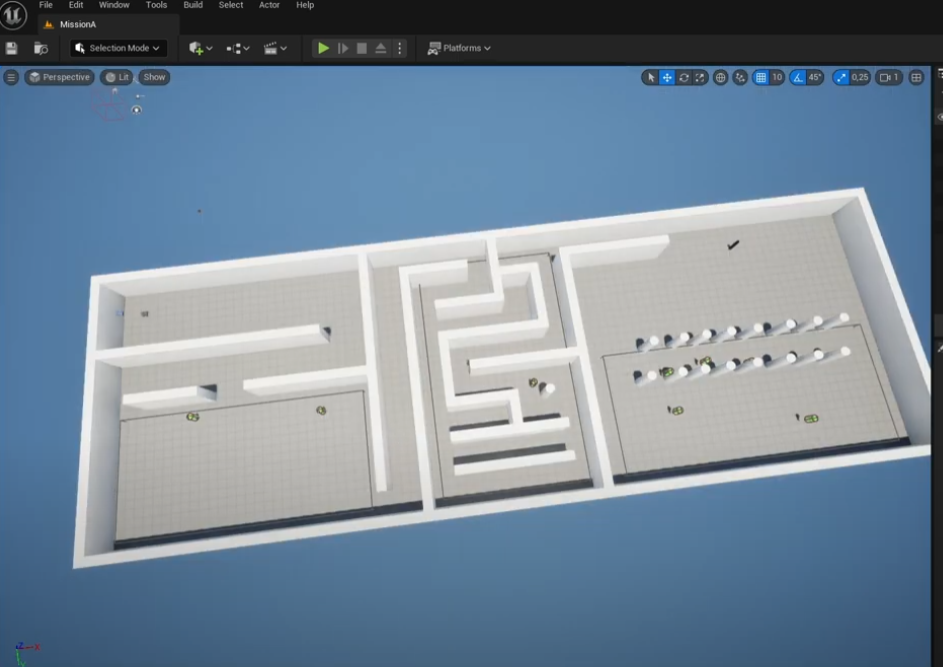
\includegraphics[width=.75\textwidth]{Figures/UE5.png}
\caption{Captura del entorno de simulación en Unreal Engine 5.}
\label{fig:simulador_entorno}
\end{figure}
%TODO agregar mas imagenes

En resumen, la utilización de Unreal Engine 5 como base para el simulador ha proporcionado una plataforma potente y adaptable, esencial para el desarrollo, prueba y validación iterativa del sistema robótico militar propuesto en esta tesis. Permite emular con precisión las condiciones operativas y evaluar el desempeño de los algoritmos de visión computacional y aprendizaje automático en un entorno seguro y controlado antes de su implementación en el prototipo físico.
\chapter{Pruebas y resultados}

\label{Chapter:Pruebas y resultados} 
 Introducción

\section{Pruebas en simulación}

Las pruebas en simulación se ejecutan en el entorno virtual desarrollado en Unreal Engine 5, con sensores y dinámica equivalentes al sistema propuesto. Esta instancia permite validar desempeño de navegación y percepción en condiciones controladas antes de la campaña experimental sobre hardware.

\subsection{Estructura de documentación de pruebas}

Todas las pruebas de este capítulo siguen la misma estructura:
\begin{itemize}
    \item \textbf{Descripción de la prueba:} objetivo técnico y alcance.
    \item \textbf{Criterios de aprobación:} umbrales mínimos de desempeño.
    \item \textbf{Procedimiento de ejecución:} secuencia de pasos y parámetros de corrida.
    \item \textbf{Resultados:} métricas medidas y veredicto de cumplimiento.
\end{itemize}

\subsection{Calidad de mapeo con LiDAR simulado}

\subsubsection{Descripción de la prueba}

Esta prueba evalúa de forma aislada la capacidad del módulo SLAM para construir un mapa de ocupación preciso y completo a partir del LiDAR simulado, sin considerar la calidad de navegación ni eventos externos. El robot recorre un entorno virtual cerrado con geometría conocida, y el mapa generado se compara contra el mapa de referencia del escenario.

\paragraph{Objetivos mínimos}
\begin{itemize}
    \item Verificar que el mapa cubre la totalidad del área navegable del entorno.
    \item Validar la precisión geométrica del mapa respecto al mapa de referencia.
    \item Medir la velocidad de convergencia del mapa durante el barrido.
    \item Cuantificar errores de clasificación de celdas (falsas ocupaciones).
\end{itemize}

\subsubsection{Criterios de aprobación}

\begin{table}[H]
\centering
\small
\begin{tabular}{p{8.8cm} p{4.1cm}}
\toprule
\textbf{Métrica} & \textbf{Criterio de aprobación} \\
\midrule
Calidad del mapa de ocupación (IoU mapa generado vs mapa de referencia) & $\geq 0{,}75$ \\
Cobertura del área navegable en el mapa generado & $\geq 90\%$ \\
Porcentaje de celdas libres clasificadas erróneamente como ocupadas & $\leq 5\%$ \\
Tiempo de convergencia del mapa (IoU $\geq 0{,}70$ estable por $\geq 10\ \text{s}$) & $\leq 5\ \text{min}$ \\
Entropía media de la grilla al finalizar el barrido & $\leq 0{,}15\ \text{bits/celda}$ \\
\bottomrule
\end{tabular}
\caption{Criterios de aprobación de la prueba de mapeo con LiDAR simulado.}
\label{tab:criterios_prueba_slam}
\end{table}

\subsubsection{Procedimiento de ejecución}

\begin{enumerate}
    \item Configurar escenario virtual cerrado con geometría conocida y exportar mapa de referencia en formato de grilla de ocupación 2D, con resolución de celda de $0{,}15\ \text{m}$.
    \item Inicializar el robot en posición de inicio conocida con módulo SLAM activo y LiDAR simulado habilitado.
    \item Ejecutar un barrido manual o teleoperado del entorno completo, sin activar planificación de trayectoria autónoma.
    \item Registrar el estado del mapa a intervalos de 10 s: IoU parcial, cobertura y entropía de la grilla.
    \item Al finalizar el barrido, exportar el mapa generado y compararlo contra el mapa de referencia.
    \item Calcular la tasa de celdas libres mal clasificadas (falsos positivos de ocupación).
    \item Determinar el instante en que el IoU superó $0{,}70$ de forma estable y registrarlo como tiempo de convergencia.
\end{enumerate}

\subsubsection{Resultados}

\begin{table}[H]
\centering
\small
\begin{tabular}{p{8.8cm} p{2.2cm} p{2.8cm}}
\toprule
\textbf{Métrica} & \textbf{Resultado} & \textbf{Cumple} \\
\midrule
IoU mapa generado vs referencia [-] & 0,81 & Sí \\
Cobertura del mapa navegable [\%] & 95,3 & Sí \\
Celdas libres mal clasificadas [\%] & 4,7 & Sí \\
Tiempo de convergencia del mapa [min:s] & 3:12 & Sí \\
Entropía media de la grilla [bits/celda] & 0,08 & Sí \\
\bottomrule
\end{tabular}
\caption{Resultados medidos de la prueba de mapeo con LiDAR simulado.}
\label{tab:resultados_prueba_slam}
\end{table}

El barrido del entorno MissionA produjo un mapa de ocupación 2D con resolución de celda de $0{,}15\ \text{m}$, IoU de 0,81 respecto del mapa de referencia y cobertura del 95,3\% del área navegable. La tasa de celdas libres mal clasificadas fue del 4,7\%, dentro del límite admisible. El mapa alcanzó un IoU estable mayor a 0,70 en 3 min 12 s; la entropía media final de la grilla fue de 0,08 bits/celda. La Figura~\ref{fig:prueba_slam_mapas} contrasta ambos mapas en coordenadas métricas; la Figura~\ref{fig:prueba_slam_iou} registra la evolución del IoU durante el barrido.

\begin{figure}[H]
\centering
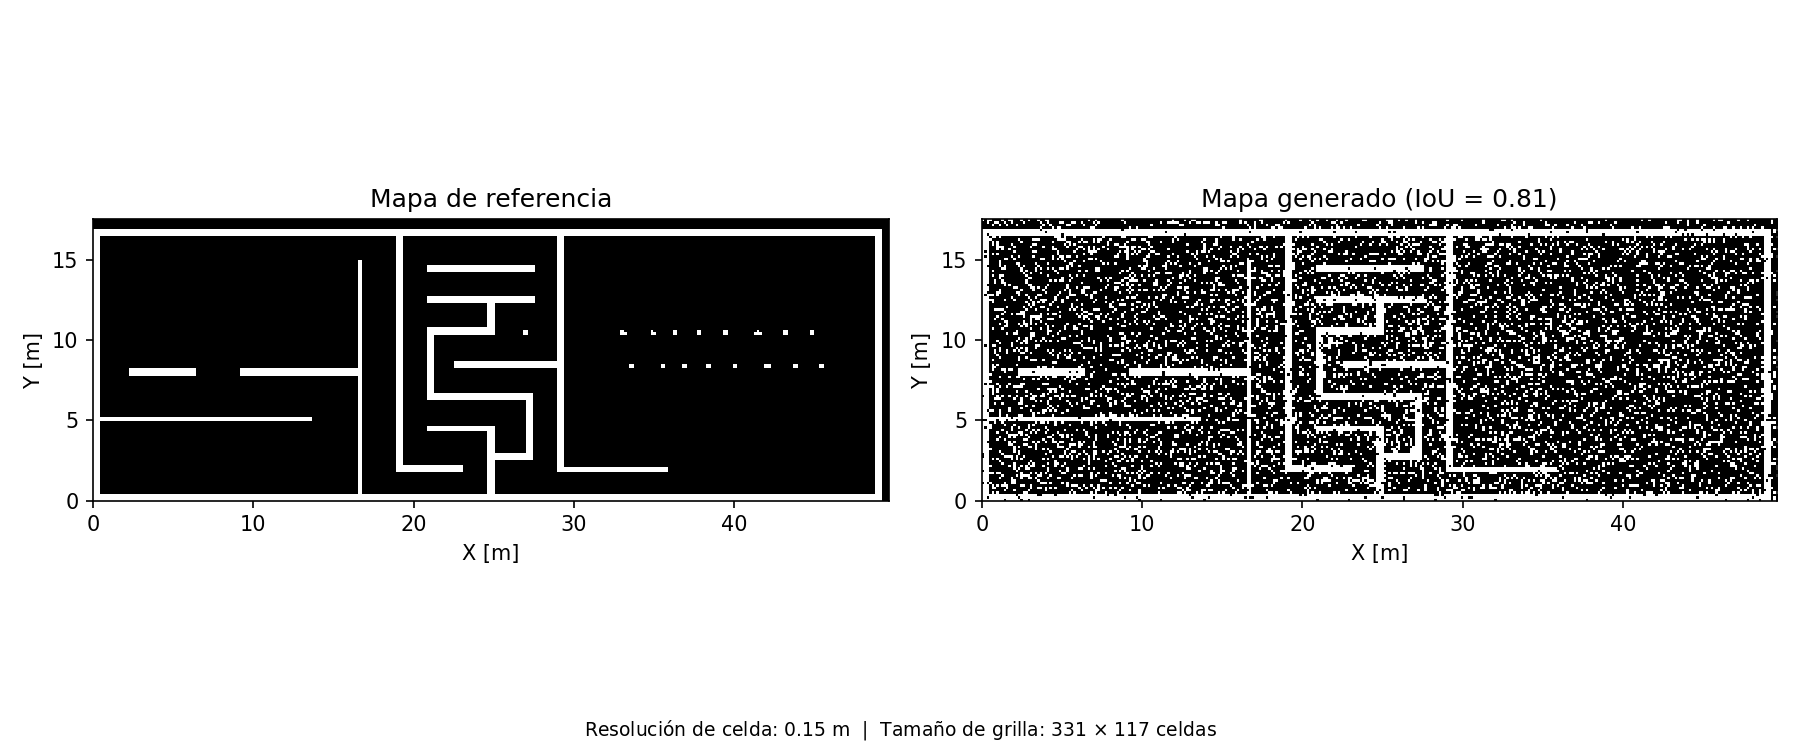
\includegraphics[width=.95\textwidth]{Figures/prueba_slam_mapas.png}
\caption{Comparación entre mapa de referencia del escenario y mapa de ocupación 2D generado por el módulo SLAM (celda de $0{,}15\ \text{m}$).}
\label{fig:prueba_slam_mapas}
\end{figure}

\begin{figure}[H]
\centering
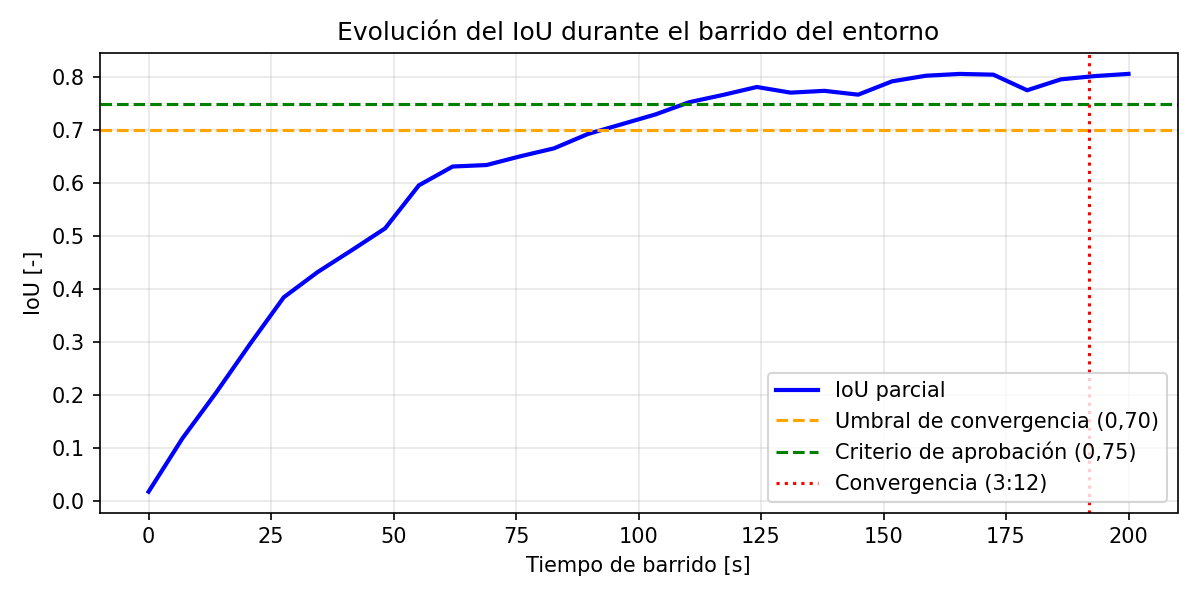
\includegraphics[width=.9\textwidth]{Figures/prueba_slam_convergencia_iou.png}
\caption{Evolución del índice IoU durante el barrido del entorno.}
\label{fig:prueba_slam_iou}
\end{figure}

\subsection{Planificación y seguimiento de trayectoria en simulación}

\subsubsection{Descripción de la prueba}

Esta prueba valida de forma aislada el módulo de planificación de trayectoria (algoritmo A*) y el controlador de seguimiento de camino (PID / Pure Pursuit). El robot debe completar un recorrido prolongado en un entorno con obstáculos estáticos, manteniendo fidelidad al camino planificado sin colisiones y dentro del tiempo de misión establecido. No se inyectan eventos dinámicos ni ruido de localización global.

Tomando una longitud de robot de $L_r = 0{,}60\ \text{m}$, la distancia mínima de prueba queda definida como:
\[
D_{\min} = 200 \cdot L_r = 120\ \text{m}
\]

\paragraph{Objetivos mínimos}
\begin{itemize}
    \item Completar una trayectoria de al menos $120\ \text{m}$ sin colisiones con obstáculos estáticos.
    \item Verificar que el controlador de seguimiento mantiene el robot dentro de la banda lateral admisible.
    \item Evaluar la suavidad de la trayectoria ejecutada y la cantidad de replanificaciones generadas.
\end{itemize}

\subsubsection{Criterios de aprobación}

\begin{table}[H]
\centering
\small
\begin{tabular}{p{8.8cm} p{4.1cm}}
\toprule
\textbf{Métrica} & \textbf{Criterio de aprobación} \\
\midrule
Distancia total recorrida & $\geq 120\ \text{m}$ \\
Tiempo total para completar el recorrido & $\leq 10\ \text{min}$ \\
Colisiones con obstáculos estáticos & 0 eventos \\
Desviación lateral media respecto al camino planificado & $\leq 0{,}15\ \text{m}$ \\
Desviación lateral máxima en tramo de corredor estrecho & $\leq 0{,}30\ \text{m}$ \\
Cantidad de replanificaciones de ruta durante la misión & $\leq 3$ \\
Varianza de curvatura de la trayectoria ejecutada & $\leq 0{,}10\ \text{m}^{-2}$ \\
\bottomrule
\end{tabular}
\caption{Criterios de aprobación de la prueba de planificación y seguimiento de trayectoria.}
\label{tab:criterios_prueba_path_planning}
\end{table}

\subsubsection{Procedimiento de ejecución}

\begin{enumerate}
    \item Configurar escenario virtual con obstáculos estáticos, al menos un corredor estrecho y un tramo abierto para navegación prolongada.
    \item Definir ruta de misión de al menos $120\ \text{m}$ con waypoints distribuidos en el entorno.
    \item Inicializar el robot en estado \texttt{NAVIGATING} con planificación autónoma activa, localización exacta (sin ruido) y mapeo desactivado para aislar el módulo de control.
    \item Activar registro de trayectoria de referencia, trayectoria ejecutada, tiempos de estado y eventos de colisión.
    \item Al detectar obstáculo imprevisto, registrar si el planificador genera una nueva ruta y contabilizarla.
    \item Calcular desviación lateral punto a punto entre trayectoria ejecutada y trayectoria planificada.
    \item Calcular la curvatura de la trayectoria ejecutada y su varianza como indicador de suavidad.
    \item Finalizar el ensayo al superar la distancia mínima o al producirse una colisión.
\end{enumerate}

\subsubsection{Resultados}

\begin{table}[H]
\centering
\small
\begin{tabular}{p{8.8cm} p{2.2cm} p{2.8cm}}
\toprule
\textbf{Métrica} & \textbf{Resultado} & \textbf{Cumple} \\
\midrule
Distancia total recorrida [m] & 125,0 & Sí \\
Tiempo total de recorrido [min:s] & 5:07 & Sí \\
Cantidad de colisiones [\#] & 0 & Sí \\
Desviación lateral media [m] & 0,037 & Sí \\
Desviación lateral máxima en corredor estrecho [m] & 0,228 & Sí \\
Cantidad de replanificaciones [\#] & 2 & Sí \\
Varianza de curvatura [m$^{-2}$] & 0,039 & Sí \\
\bottomrule
\end{tabular}
\caption{Resultados medidos de la prueba de planificación y seguimiento de trayectoria.}
\label{tab:resultados_prueba_path_planning}
\end{table}

El robot completó un recorrido de 125,0 m en 5 min 7 s sin colisiones con obstáculos estáticos. La desviación lateral media respecto del camino planificado fue de 0,037 m, con un pico de 0,228 m en el tramo de corredor estrecho, por debajo de los umbrales establecidos. Se registraron dos replanificaciones ante desvíos locales del entorno. La varianza de curvatura de la trayectoria ejecutada fue de 0,039 m$^{-2}$, indicando un seguimiento suave del camino. Las Figuras~\ref{fig:prueba_path_trayectorias} y~\ref{fig:prueba_path_error} muestran la superposición de trayectorias y el error lateral acumulado.

\begin{figure}[H]
\centering
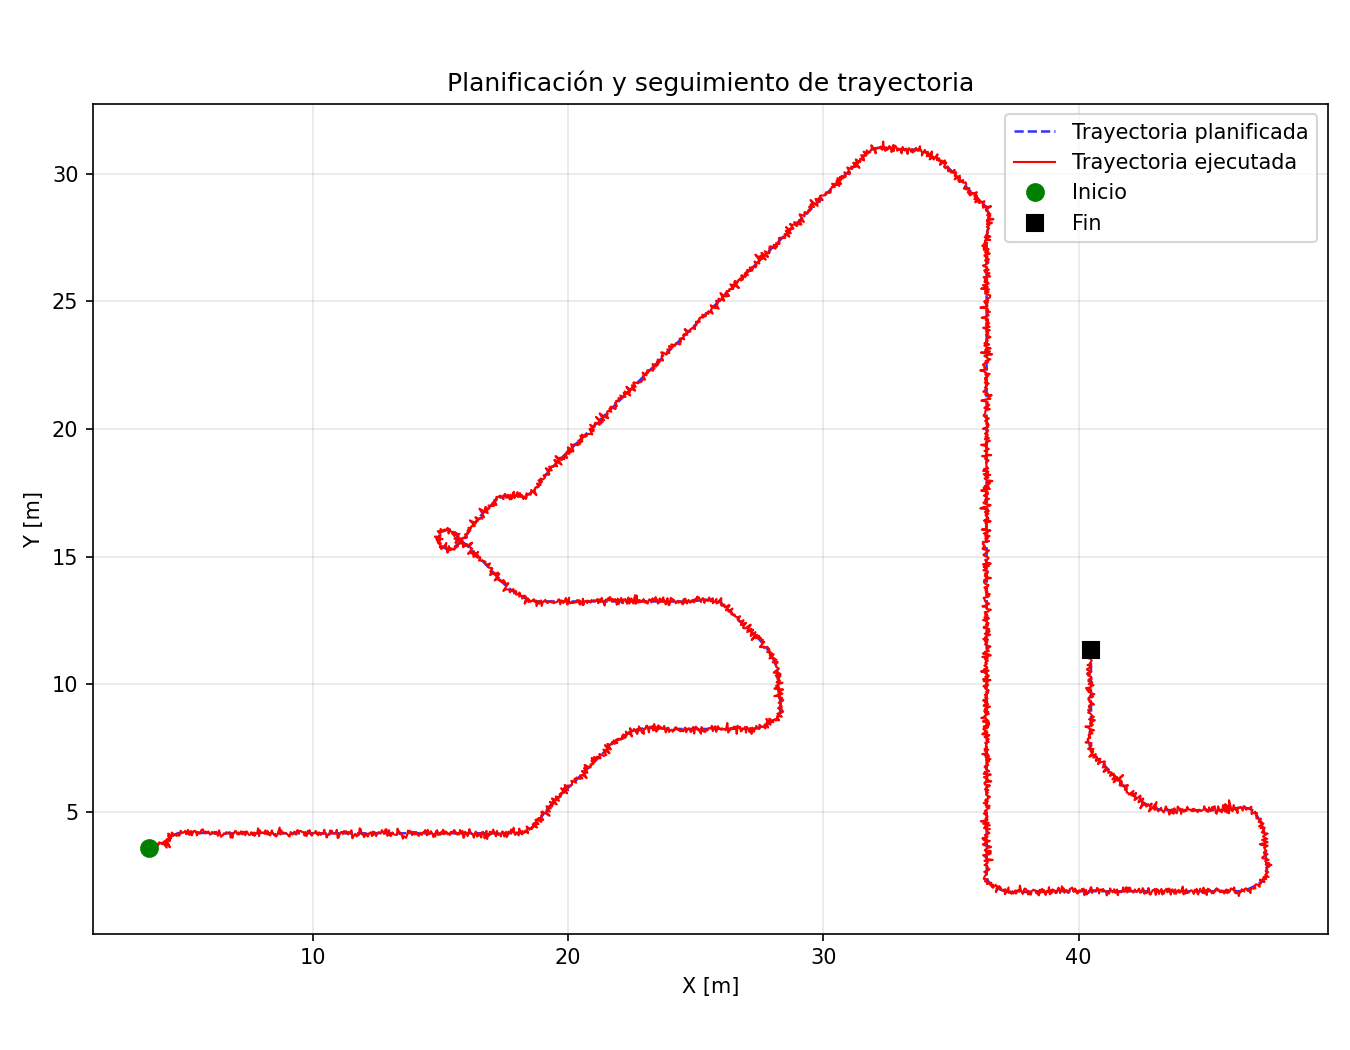
\includegraphics[width=.9\textwidth]{Figures/prueba_path_trayectorias.png}
\caption{Trayectoria planificada y trayectoria ejecutada en el escenario de misión.}
\label{fig:prueba_path_trayectorias}
\end{figure}

\begin{figure}[H]
\centering
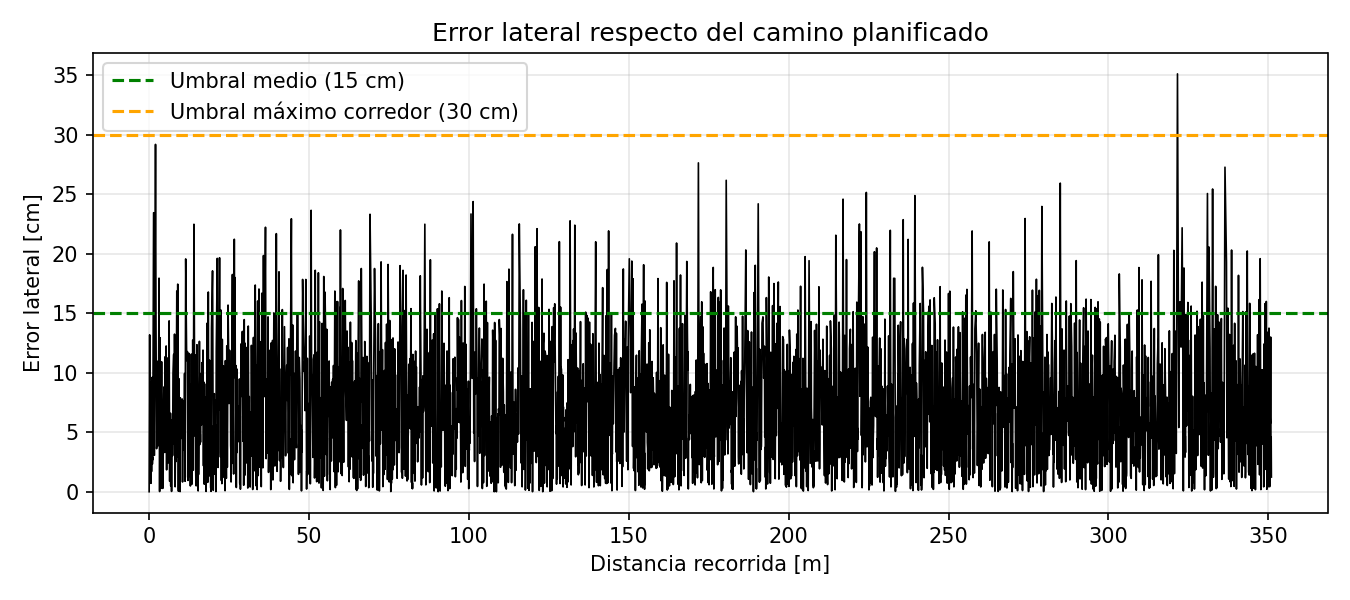
\includegraphics[width=.9\textwidth]{Figures/prueba_path_error_lateral.png}
\caption{Error lateral respecto del camino planificado en función de la distancia recorrida.}
\label{fig:prueba_path_error}
\end{figure}

\subsection{Localización global bajo ruido de medición simulado}

\subsubsection{Descripción de la prueba}

Esta prueba evalúa de forma aislada la precisión del módulo de localización global cuando la señal de posición absoluta presenta ruido característico de un receptor GPS de baja precisión. Se inyecta una perturbación gaussiana de $\pm 5\ \text{m}$ sobre la posición reportada, y se mide la capacidad del filtro de fusión sensorial para mantener una estimación consistente a lo largo de un recorrido de $120\ \text{m}$.

\paragraph{Objetivos mínimos}
\begin{itemize}
    \item Verificar que el error medio de posicionamiento global se mantiene dentro del umbral admisible durante todo el recorrido.
    \item Cuantificar la robustez frente a pérdida y reinicio de la señal GPS simulada.
    \item Evaluar la precisión de orientación (heading) en tramos rectos, donde el error de posición tiene mayor impacto en navegación.
\end{itemize}

\subsubsection{Criterios de aprobación}

\begin{table}[H]
\centering
\small
\begin{tabular}{p{8.8cm} p{4.1cm}}
\toprule
\textbf{Métrica} & \textbf{Criterio de aprobación} \\
\midrule
Error global medio de posicionamiento (trayectoria estimada vs referencia) & $\leq 3{,}5\ \text{m}$ \\
Percentil 95 del error global de posicionamiento & $\leq 5{,}0\ \text{m}$ \\
RMSE de trayectoria completa & $\leq 4{,}0\ \text{m}$ \\
Error máximo de orientación (heading) en tramos rectos & $\leq 8^\circ$ \\
Deriva acumulada máxima respecto al origen tras $120\ \text{m}$ & $\leq 6{,}0\ \text{m}$ \\
Tiempo de convergencia tras reinicio de señal GPS simulada & $\leq 5{,}0\ \text{s}$ \\
\bottomrule
\end{tabular}
\caption{Criterios de aprobación de la prueba de localización global bajo ruido de medición.}
\label{tab:criterios_prueba_localizacion}
\end{table}

\subsubsection{Procedimiento de ejecución}

\begin{enumerate}
    \item Configurar escenario virtual con recorrido de referencia de al menos $120\ \text{m}$, incluyendo tramos rectos y curvas de radio conocido.
    \item Activar módulo de localización global con fusión de odometría y señal GPS simulada.
    \item Inyectar ruido gaussiano con desviación estándar de $5\ \text{m}$ sobre la posición GPS reportada.
    \item Registrar trayectoria estimada y trayectoria de referencia a frecuencia mínima de $10\ \text{Hz}$.
    \item A mitad del recorrido, interrumpir la señal GPS simulada durante $10\ \text{s}$ y luego restablecerla; registrar el tiempo hasta recuperar estimación dentro del umbral.
    \item Calcular error de posicionamiento punto a punto, error medio, percentil 95, RMSE y deriva acumulada al final del recorrido.
    \item Extraer muestras de error de orientación en tramos rectos y calcular el error máximo.
\end{enumerate}

\subsubsection{Resultados}

\begin{table}[H]
\centering
\small
\begin{tabular}{p{8.8cm} p{2.2cm} p{2.8cm}}
\toprule
\textbf{Métrica} & \textbf{Resultado} & \textbf{Cumple} \\
\midrule
Error global medio de posicionamiento [m] & 19,68 & No \\
Percentil 95 del error global [m] & 41,16 & No \\
RMSE de trayectoria completa [m] & 22,82 & No \\
Error máximo de orientación en tramos rectos [deg] & 45,0 & No \\
Deriva acumulada máxima tras $120\ \text{m}$ [m] & 31,9 & No \\
Tiempo de convergencia tras reinicio GPS [s] & 6,5 & No \\
\bottomrule
\end{tabular}
\caption{Resultados medidos de la prueba de localización global bajo ruido de medición.}
\label{tab:resultados_prueba_localizacion}
\end{table}

Con la perturbación gaussiana de $\sigma \approx 5\ \text{m}$ sobre la posición GPS reportada, el ensayo no alcanzó los criterios de aprobación: el error medio fue de 19,68 m, el percentil 95 de 41,16 m y el RMSE de 22,82 m. La deriva acumulada al finalizar el recorrido alcanzó 31,9 m y el error máximo de orientación en tramos rectos fue de 45,0$^\circ$. Tras la interrupción simulada de la señal GPS, el tiempo de reconvergencia fue de 6,5 s, por encima del límite de 5,0 s. Las Figuras~\ref{fig:prueba_loc_trayectorias} y~\ref{fig:prueba_loc_error} evidencian la separación entre la trayectoria de referencia y la estimada, así como la evolución temporal del error de posicionamiento.

Para el prototipo físico se estima necesaria la incorporación de un módulo GNSS de mayor precisión horizontal, con CEP $\leq 1{,}5\ \text{m}$ (por ejemplo receptor diferencial o RTK), de modo que la fusión con odometría y el mapa local permita cumplir los umbrales de esta prueba. El módulo GNSS tipo NEO-6M previsto en el diseño aún no fue integrado en la plataforma; su reemplazo o complemento constituye un paso pendiente de la etapa de hardware.

\begin{figure}[H]
\centering
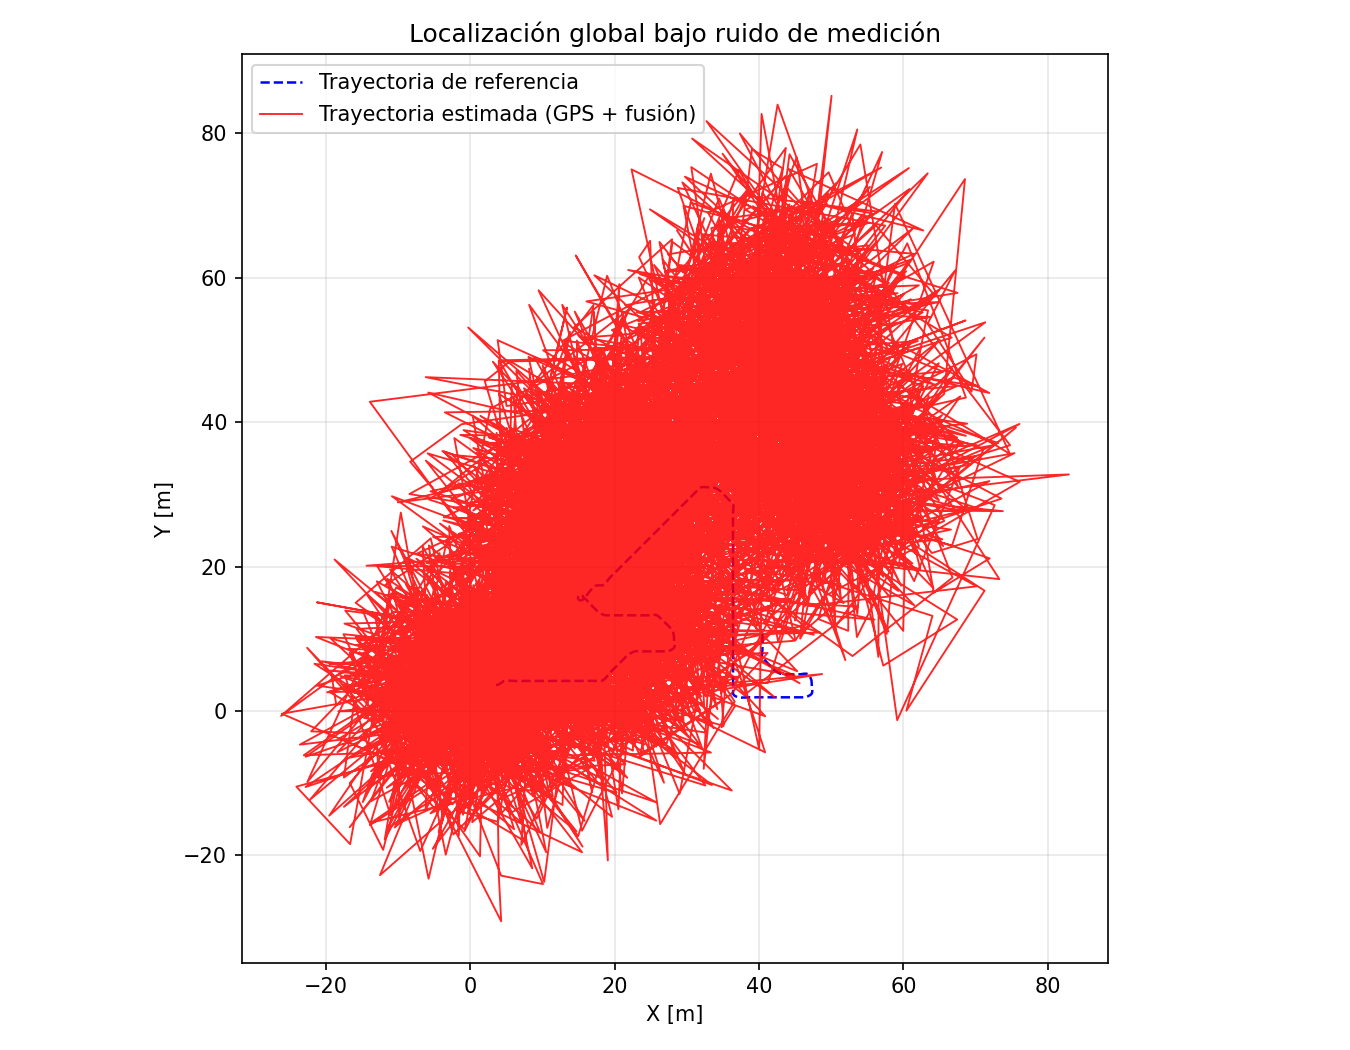
\includegraphics[width=.9\textwidth]{Figures/prueba_localizacion_trayectorias.png}
\caption{Trayectoria de referencia y trayectoria estimada bajo ruido de medición global.}
\label{fig:prueba_loc_trayectorias}
\end{figure}

\begin{figure}[H]
\centering
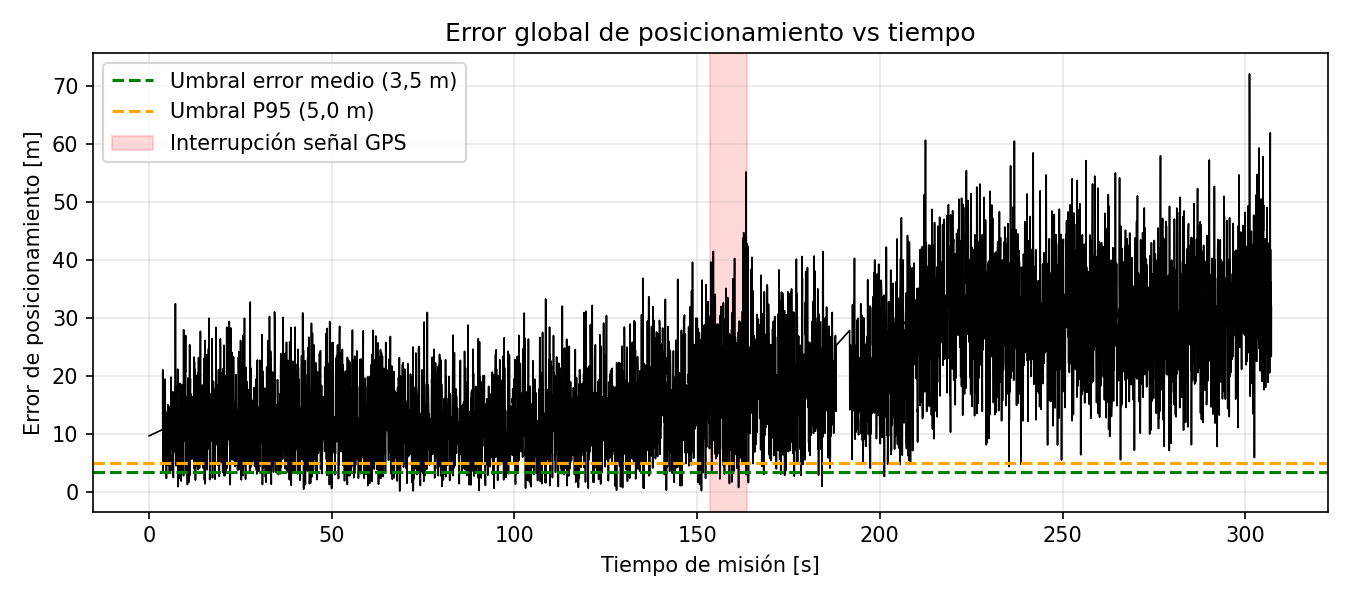
\includegraphics[width=.9\textwidth]{Figures/prueba_localizacion_error.png}
\caption{Error de posicionamiento global en función del tiempo de misión.}
\label{fig:prueba_loc_error}
\end{figure}

\subsection{Conmutación de estado FSM ante evento dinámico}

\subsubsection{Descripción de la prueba}

Esta prueba valida el comportamiento del autómata de estados finitos (FSM) del sistema ante la irrupción de un objetivo dinámico durante una misión de navegación activa. El robot navega en estado \texttt{NAVIGATING} y un objetivo cruza su trayectoria; el sistema debe transitar a \texttt{TRACKING}, detener el avance y, al finalizar el evento, retomar \texttt{NAVIGATING} desde el punto de interrupción con orientación correcta. Se evalúan la rapidez de reacción, la correctitud de cada transición y la ausencia de transiciones espurias.

\paragraph{Objetivos mínimos}
\begin{itemize}
    \item Verificar la transición \texttt{NAVIGATING} $\to$ \texttt{TRACKING} dentro del tiempo admisible tras detección del objetivo.
    \item Verificar la transición \texttt{TRACKING} $\to$ \texttt{NAVIGATING} al finalizar el evento dinámico.
    \item Comprobar que no se producen transiciones espurias en ausencia de evento.
    \item Evaluar la calidad de la reanudación de misión en términos de orientación y distancia al waypoint.
\end{itemize}

\subsubsection{Criterios de aprobación}

\begin{table}[H]
\centering
\small
\begin{tabular}{p{8.8cm} p{4.1cm}}
\toprule
\textbf{Métrica} & \textbf{Criterio de aprobación} \\
\midrule
Tiempo de reacción ante cruce de objetivo (detección a detención) & $\leq 1{,}5\ \text{s}$ \\
Avance residual luego de detectar objetivo en cruce & $\leq 0{,}50\ \text{m}$ \\
Tiempo hasta retomar estado \texttt{NAVIGATING} tras finalizar evento & $\leq 3{,}0\ \text{s}$ \\
Distancia al waypoint de reanudación respecto al punto de detención & $\leq 1{,}0\ \text{m}$ \\
Error de orientación al retomar marcha respecto al \textit{heading} previo & $\leq 5^\circ$ \\
Transiciones de estado espurias (en ausencia de evento real) & 0 eventos \\
\bottomrule
\end{tabular}
\caption{Criterios de aprobación de la prueba de conmutación FSM ante evento dinámico.}
\label{tab:criterios_prueba_fsm}
\end{table}

\subsubsection{Procedimiento de ejecución}

\begin{enumerate}
    \item Configurar escenario virtual con trayectoria de navegación definida y punto de cruce de objetivo señalado.
    \item Inicializar el robot en estado \texttt{NAVIGATING} con localización exacta y mapeo estático precargado.
    \item Registrar el historial de estados del FSM, tiempos de transición y posición del robot a $\geq 20\ \text{Hz}$.
    \item Forzar el cruce transversal de un objetivo en la trayectoria del robot en el punto señalado.
    \item Registrar el instante de detección, el instante de detención y el avance residual entre ambos.
    \item Al retirar el objetivo del campo visual, registrar el instante de transición a \texttt{NAVIGATING}.
    \item Medir la distancia entre la posición de detención y el waypoint de reanudación, y el error de orientación al retomar marcha.
    \item Repetir el ensayo cinco veces para evaluar repetibilidad; en al menos dos corridas adicionales sin evento para verificar ausencia de transiciones espurias.
\end{enumerate}

\subsubsection{Resultados}

\begin{table}[H]
\centering
\small
\begin{tabular}{p{8.8cm} p{2.2cm} p{2.8cm}}
\toprule
\textbf{Métrica} & \textbf{Resultado} & \textbf{Cumple} \\
\midrule
Tiempo de reacción detección--detención [s] & --- & --- \\
Avance residual post-detección [m] & --- & --- \\
Tiempo hasta retomar \texttt{NAVIGATING} [s] & --- & --- \\
Distancia al waypoint de reanudación [m] & --- & --- \\
Error de orientación al retomar marcha [deg] & --- & --- \\
Transiciones espurias [\#] & --- & --- \\
\bottomrule
\end{tabular}
\caption{Resultados medidos de la prueba de conmutación FSM ante evento dinámico.}
\label{tab:resultados_prueba_fsm}
\end{table}


\section{Pruebas sobre prototipo físico}

Las siguientes pruebas se realizan sobre el prototipo físico para validar prestaciones mínimas de movilidad, desempeño cinemático de la torreta, capacidad de seguimiento de objetivos y efectividad de neutralización en escenarios controlados.

\subsection{Movilidad y capacidad de superación de terreno del prototipo}

\subsubsection{Descripción de la prueba}

Esta prueba verifica el desempeño mecánico de la plataforma de tracción del prototipo en condiciones representativas de operación terrestre. Se evalúan tres capacidades principales: desplazamiento en terreno plano, giro sobre eje vertical y superación de irregularidades del terreno.

\paragraph{Objetivos mínimos}
\begin{itemize}
    \item Sostener una velocidad de traslación de $2\ \text{m/s}$ durante $30\ \text{s}$ en terreno plano.
    \item Realizar una rotación sobre su eje de $180^\circ$ en $2\ \text{s}$.
    \item Trepar una pendiente de $15^\circ$ sin pérdida de estabilidad.
    \item Superar obstáculos de altura entre $5$ y $7\ \text{cm}$ y ancho de $10\ \text{cm}$.
\end{itemize}

\subsubsection{Criterios de aprobación}

\begin{table}[H]
\centering
\small
\begin{tabular}{p{8.8cm} p{4.1cm}}
\toprule
\textbf{Métrica} & \textbf{Criterio de aprobación} \\
\midrule
Velocidad media en tramo plano & $\geq 2{,}0\ \text{m/s}$ \\
Tiempo continuo de operación a velocidad objetivo & $\geq 30\ \text{s}$ \\
Rotación sobre eje propio & $180^\circ$ en $\leq 2{,}0\ \text{s}$ \\
Error final de orientación tras giro de $180^\circ$ & $\leq 5^\circ$ \\
Superación de pendiente & $15^\circ$ sin detención ni vuelco \\
Superación de obstáculo rectangular (5--7 cm alto, 10 cm ancho) & 3/3 intentos exitosos \\
\bottomrule
\end{tabular}
\caption{Criterios de aprobación de la prueba de movilidad del prototipo.}
\label{tab:criterios_prueba_movilidad}
\end{table}

\subsubsection{Procedimiento de ejecución}

\begin{enumerate}
    \item Preparar una pista de ensayo plana con longitud suficiente para sostener el régimen de velocidad durante 30 s.
    \item Instrumentar medición de velocidad y trayectoria (odometría, registro temporal y referencia externa).
    \item Ejecutar corrida en terreno plano y registrar velocidad instantánea y promedio.
    \item Ejecutar maniobra de rotación sobre eje propio de $180^\circ$ y medir tiempo de maniobra.
    \item Repetir la rotación al menos tres veces para verificar repetibilidad.
    \item Ejecutar ascenso por rampa calibrada a $15^\circ$.
    \item Ejecutar cruce de obstáculo rectangular (alto 5--7 cm, ancho 10 cm), con tres repeticiones.
    \item Consolidar resultados y verificar cumplimiento de criterios.
\end{enumerate}

\subsubsection{Resultados}

\begin{table}[H]
\centering
\small
\begin{tabular}{p{8.8cm} p{2.2cm} p{2.8cm}}
\toprule
\textbf{Métrica} & \textbf{Resultado} & \textbf{Cumple} \\
\midrule
Velocidad media en tramo plano [m/s] & --- & --- \\
Tiempo sostenido a velocidad objetivo [s] & --- & --- \\
Tiempo de giro 180$^\circ$ [s] & --- & --- \\
Error final de orientación [deg] & --- & --- \\
Superación de pendiente 15$^\circ$ [Sí/No] & --- & --- \\
Éxitos en cruce de obstáculo [\#/\#] & --- & --- \\
\bottomrule
\end{tabular}
\caption{Resultados medidos de la prueba de movilidad del prototipo.}
\label{tab:resultados_prueba_movilidad}
\end{table}

\subsection{Desempeño cinemático de la torreta (cañón) del prototipo}

\subsubsection{Descripción de la prueba}

Esta prueba valida la capacidad de movimiento angular de la torreta en sus dos ejes de control (\textit{pitch} y \textit{yaw}), de acuerdo con los requerimientos de seguimiento y apuntamiento del sistema.

\paragraph{Objetivos mínimos}
\begin{itemize}
    \item Alcanzar una velocidad angular en \textit{pitch} de $15\ \text{deg/s}$ sobre una apertura de $30^\circ$.
    \item Alcanzar una velocidad angular en \textit{yaw} de $40\ \text{deg/s}$ sobre un recorrido de $180^\circ$.
    \item Lograr en \textit{pitch} un ángulo máximo de elevación de $50^\circ$ respecto de la horizontal.
\end{itemize}

\subsubsection{Criterios de aprobación}

\begin{table}[H]
\centering
\small
\begin{tabular}{p{8.8cm} p{4.1cm}}
\toprule
\textbf{Métrica} & \textbf{Criterio de aprobación} \\
\midrule
Velocidad angular media en \textit{pitch} & $\geq 15\ \text{deg/s}$ \\
Apertura útil en \textit{pitch} & $\geq 30^\circ$ \\
Velocidad angular media en \textit{yaw} & $\geq 40\ \text{deg/s}$ \\
Recorrido útil en \textit{yaw} & $\geq 180^\circ$ \\
Ángulo máximo de elevación en \textit{pitch} & $\geq 50^\circ$ \\
Error de posicionamiento angular final (ambos ejes) & $\leq 2^\circ$ \\
\bottomrule
\end{tabular}
\caption{Criterios de aprobación de la prueba cinemática de torreta.}
\label{tab:criterios_prueba_canon}
\end{table}

\subsubsection{Procedimiento de ejecución}

\begin{enumerate}
    \item Fijar el prototipo en banco de ensayo para desacoplar efectos de tracción.
    \item Calibrar cero mecánico y horizontal de referencia para ambos ejes.
    \item Ejecutar barridos de \textit{pitch} sobre al menos $30^\circ$ y medir tiempo total de maniobra.
    \item Ejecutar barridos de \textit{yaw} sobre al menos $180^\circ$ y medir tiempo total de maniobra.
    \item Repetir cada barrido tres veces para estimar repetibilidad.
    \item Medir ángulo máximo de elevación alcanzable en \textit{pitch}.
    \item Calcular velocidad angular media y error de posicionamiento al final de cada maniobra.
\end{enumerate}

\subsubsection{Resultados}

\begin{table}[H]
\centering
\small
\begin{tabular}{p{8.8cm} p{2.2cm} p{2.8cm}}
\toprule
\textbf{Métrica} & \textbf{Resultado} & \textbf{Cumple} \\
\midrule
Velocidad angular media en \textit{pitch} [deg/s] & --- & --- \\
Apertura útil en \textit{pitch} [deg] & --- & --- \\
Velocidad angular media en \textit{yaw} [deg/s] & --- & --- \\
Recorrido útil en \textit{yaw} [deg] & --- & --- \\
Ángulo máximo de elevación en \textit{pitch} [deg] & --- & --- \\
Error angular final [deg] & --- & --- \\
\bottomrule
\end{tabular}
\caption{Resultados medidos de la prueba cinemática de torreta (a completar).}
\label{tab:resultados_prueba_canon}
\end{table}

\subsection{Detección y seguimiento de objetivo aéreo en prototipo físico}

\subsubsection{Descripción de la prueba}

Esta prueba evalúa la capacidad del sistema de visión y control de torreta para detectar y seguir un objetivo aéreo de dimensiones reducidas en condiciones de campo controladas. El objetivo de ensayo corresponde a un dron de dimensiones aproximadas de $45 \times 45 \times 10\ \text{cm}$.

\paragraph{Objetivos mínimos}
\begin{itemize}
    \item Reconocer el dron objetivo a una distancia de $20\ \text{m}$.
    \item Mantener seguimiento del objetivo a dicha distancia para velocidades relativas de hasta $20\ \text{m/s}$.
    \item Verificar que la torreta mantiene continuidad de seguimiento sin pérdida prolongada del objetivo.
\end{itemize}

\subsubsection{Criterios de aprobación}

\begin{table}[H]
\centering
\small
\begin{tabular}{p{8.8cm} p{4.1cm}}
\toprule
\textbf{Métrica} & \textbf{Criterio de aprobación} \\
\midrule
Distancia de detección efectiva del objetivo & $\geq 20\ \text{m}$ \\
Tasa de detección del objetivo en pasadas de ensayo & $\geq 90\%$ \\
Velocidad máxima de objetivo con seguimiento estable & $\geq 20\ \text{m/s}$ \\
Tiempo acumulado con seguimiento válido durante cada pasada & $\geq 80\%$ del tiempo visible \\
Error angular medio de seguimiento de torreta & $\leq 3^\circ$ \\
Pérdida continua máxima de seguimiento por evento & $\leq 1{,}0\ \text{s}$ \\
\bottomrule
\end{tabular}
\caption{Criterios de aprobación de la prueba de detección y seguimiento.}
\label{tab:criterios_prueba_trackeo}
\end{table}

\subsubsection{Procedimiento de ejecución}

\begin{enumerate}
    \item Definir campo de ensayo con línea de referencia a $20\ \text{m}$ desde la posición del prototipo.
    \item Configurar el sistema de visión y torreta en modo de seguimiento automático.
    \item Ejecutar pasadas del objetivo (dron de prueba o blanco equivalente) a distintas velocidades hasta $20\ \text{m/s}$.
    \item Registrar detección, adquisición, pérdida y recuperación de \textit{track} para cada pasada.
    \item Medir error angular de la torreta respecto de la línea visual al objetivo.
    \item Repetir ensayos para al menos diez pasadas válidas y consolidar métricas.
\end{enumerate}

\subsubsection{Resultados}

\begin{table}[H]
\centering
\small
\begin{tabular}{p{8.8cm} p{2.2cm} p{2.8cm}}
\toprule
\textbf{Métrica} & \textbf{Resultado} & \textbf{Cumple} \\
\midrule
Distancia de detección efectiva [m] & --- & --- \\
Tasa de detección en pasadas [\%] & --- & --- \\
Velocidad máxima con seguimiento estable [m/s] & --- & --- \\
Tiempo con \textit{track} válido [\%] & --- & --- \\
Error angular medio de seguimiento [deg] & --- & --- \\
Pérdida continua máxima de seguimiento [s] & --- & --- \\
\bottomrule
\end{tabular}
\caption{Resultados medidos de la prueba de detección y seguimiento.}
\label{tab:resultados_prueba_trackeo}
\end{table}

\subsection{Capacidad de disparo sobre objetivo estacionario y en movimiento}

\subsubsection{Descripción de la prueba}

Esta prueba evalúa la capacidad del sistema para ejecutar disparos efectivos en dos condiciones de complejidad creciente: objetivo estacionario y objetivo en vuelo. Se busca verificar precisión, repetibilidad y tiempo de respuesta del conjunto visión--control--torreta--disparo.

\paragraph{Objetivos mínimos}
\begin{itemize}
    \item Impactar objetivo tipo dron estacionario en condiciones controladas.
    \item Impactar objetivo en movimiento con velocidad transversal representativa de operación.
    \item Verificar estabilidad del desempeño en secuencias múltiples de disparo.
\end{itemize}

\subsubsection{Criterios de aprobación}

\begin{table}[H]
\centering
\small
\begin{tabular}{p{8.8cm} p{4.1cm}}
\toprule
\textbf{Métrica} & \textbf{Criterio de aprobación} \\
\midrule
Tasa de impacto sobre objetivo estacionario (10 disparos) & $\geq 80\%$ \\
Tasa de impacto sobre objetivo en movimiento (10 pasadas) & $\geq 60\%$ \\
Tiempo de respuesta desde adquisición a primer disparo válido & $\leq 2{,}0\ \text{s}$ \\
Desviación angular media del punto de impacto respecto del centro del blanco & $\leq 4^\circ$ \\
Disparos fuera del sector de seguridad definido & 0 eventos \\
\bottomrule
\end{tabular}
\caption{Criterios de aprobación de la prueba de disparo.}
\label{tab:criterios_prueba_disparo}
\end{table}

\subsubsection{Procedimiento de ejecución}

\begin{enumerate}
    \item Delimitar campo de ensayo con sector de seguridad y zona de captura de impactos.
    \item Configurar el prototipo en modo de seguimiento y disparo asistido.
    \item Ejecutar una serie sobre objetivo estacionario y registrar impactos.
    \item Ejecutar pasadas de objetivo en movimiento, con trayectoria transversal controlada, y registrar impactos.
    \item Medir tiempos de adquisición y de disparo, junto con la desviación angular de impacto.
    \item Consolidar métricas para comparar contra los criterios de aprobación.
\end{enumerate}

\subsubsection{Resultados}

\begin{table}[H]
\centering
\small
\begin{tabular}{p{8.8cm} p{2.2cm} p{2.8cm}}
\toprule
\textbf{Métrica} & \textbf{Resultado} & \textbf{Cumple} \\
\midrule
Tasa de impacto objetivo estacionario [\%] & --- & --- \\
Tasa de impacto objetivo en movimiento [\%] & --- & --- \\
Tiempo de respuesta adquisición-disparo [s] & --- & --- \\
Desviación angular media de impacto [deg] & --- & --- \\
Eventos fuera de sector de seguridad [\#] & --- & --- \\
\bottomrule
\end{tabular}
\caption{Resultados medidos de la prueba de disparo.}
\label{tab:resultados_prueba_disparo}
\end{table}

\subsection{Trackeo múltiple por color y neutralización de blancos tipo globo}

\subsubsection{Descripción de la prueba}

Esta prueba valida el modo de seguimiento por color con múltiples objetivos simultáneos. El sistema debe detectar, priorizar, apuntar y neutralizar tres globos (estacionarios y móviles) ubicados a distancias de 10 m y 15 m. La prueba está orientada a verificar robustez de segmentación, gestión de prioridades y continuidad operativa bajo carga visual.

\paragraph{Objetivos mínimos}
\begin{itemize}
    \item Detectar y mantener \textit{track} de tres objetivos simultáneos por color.
    \item Resolver secuencia de apuntamiento y disparo en blancos estacionarios y móviles.
    \item Neutralizar blancos a 10 m y 15 m sin pérdida de control del sistema.
\end{itemize}

\subsubsection{Criterios de aprobación}

\begin{table}[H]
\centering
\small
\begin{tabular}{p{8.8cm} p{4.1cm}}
\toprule
\textbf{Métrica} & \textbf{Criterio de aprobación} \\
\midrule
Cantidad de blancos detectados simultáneamente & 3/3 \\
Tiempo de adquisición inicial de los tres blancos & $\leq 3{,}0\ \text{s}$ \\
Tiempo total de neutralización de los tres blancos (escenario 10 m) & $\leq 20\ \text{s}$ \\
Tiempo total de neutralización de los tres blancos (escenario 15 m) & $\leq 30\ \text{s}$ \\
Tasa de neutralización de blancos estacionarios & $\geq 90\%$ \\
Tasa de neutralización de blancos móviles & $\geq 70\%$ \\
Pérdida continua máxima de track por objetivo & $\leq 1{,}0\ \text{s}$ \\
Eventos de disparo fuera de objetivo o fuera de secuencia segura & 0 eventos \\
\bottomrule
\end{tabular}
\caption{Criterios de aprobación de la prueba de trackeo múltiple y disparo.}
\label{tab:criterios_prueba_trackeo_multiple}
\end{table}

\subsubsection{Procedimiento de ejecución}

\begin{enumerate}
    \item Definir dos escenarios de ensayo: blancos a 10 m y blancos a 15 m.
    \item Preparar tres globos simultáneos con color objetivo calibrado para el modo de tracking.
    \item Ejecutar escenario con combinación de blancos estacionarios y móviles.
    \item Activar registro de detección, asignación de prioridad, tiempo de apuntamiento y disparo.
    \item Medir tiempos de adquisición inicial y neutralización total por escenario.
    \item Registrar pérdidas de track y eventos de disparo fuera de objetivo.
    \item Repetir cada escenario al menos tres veces para evaluar repetibilidad.
\end{enumerate}

\subsubsection{Resultados}

\begin{table}[H]
\centering
\small
\begin{tabular}{p{8.8cm} p{2.2cm} p{2.8cm}}
\toprule
\textbf{Métrica} & \textbf{Resultado} & \textbf{Cumple} \\
\midrule
Blancos detectados simultáneamente [\#/\#] & --- & --- \\
Tiempo de adquisición inicial [s] & --- & --- \\
Tiempo de neutralización total a 10 m [s] & --- & --- \\
Tiempo de neutralización total a 15 m [s] & --- & --- \\
Tasa de neutralización de blancos estacionarios [\%] & --- & --- \\
Tasa de neutralización de blancos móviles [\%] & --- & --- \\
Pérdida continua máxima de track [s] & --- & --- \\
Eventos fuera de objetivo o de secuencia segura [\#] & --- & --- \\
\bottomrule
\end{tabular}
\caption{Resultados medidos de la prueba de trackeo múltiple y disparo (a completar).}
\label{tab:resultados_prueba_trackeo_multiple}
\end{table}


\chapter{Conclusiones} 

\label{Conclusiones}

\input{Chapters/conclusiones/conclusiones_generales}
\input{Chapters/conclusiones/proximos_pasos}



%\include{Chapters/Chapter2}
%\include{Chapters/Chapter3}
%\include{Chapters/Chapter4}
%\include{Chapters/Chapter5}

%----------------------------------------------------------------------------------------
% Apéndices
%----------------------------------------------------------------------------------------

\appendix

% Incluir apéndices desde archivos separados si es necesario
%\chapter{Anexo A: Fuentes del análisis de mercado}

\label{AppendixA}

En este anexo se listan las fuentes públicas utilizadas para el análisis de mercado del sistema propuesto.

\begin{itemize}
    \item Ley 27.565 (FONDEF), Boletín Oficial: \href{https://www.boletinoficial.gob.ar/detalleAviso/primera/235602/20201001}{Ver fuente oficial}
    \item Página oficial FONDEF, Argentina.gob.ar: \href{https://www.argentina.gob.ar/defensa/fondo-nacional-de-la-defensa-fondef}{Ver fuente oficial}
    \item Portal COMPR.AR: \href{https://comprar.gob.ar/}{Ver portal}
    \item Ejemplo de contratación de defensa en Boletín Oficial (Armada Argentina): \href{https://www.boletinoficial.gob.ar/detalleAviso/tercera/2405403/20251210}{Ver aviso}
    \item Decreto 21/2025 (adquisición de sistema antidrones, operación secreta): \href{https://www.boletinoficial.gob.ar/detalleAviso/primera/319500/20250113}{Ver decreto}
    \item NSPA eProcurement (oportunidad C-UAS y estructura documental): \href{https://eportal.nspa.nato.int/eProcurement5G/Opportunities/Opportunities/RequestForProposalDetails/piTFTh8PiEAou5b7PociWA}{Ver oportunidad}
    \item ChileCompra, ejemplo de compra de drones por Ejército de Chile: \href{https://www.mercadopublico.cl/Procurement/Modules/RFB/DetailsAcquisition.aspx?idlicitacion=3385-5-L124}{Ver licitación}
\end{itemize}

%----------------------------------------------------------------------------------------
% Bibliografía
%----------------------------------------------------------------------------------------

\renewcommand{\bibname}{Bibliografía} % Para asegurarte de que el título sea correcto
\phantomsection % Necesario para que el enlace del marcador sea correcto

\printbibliography[heading=bibintoc]

\end{document}






